\section{Results}

\subsection{Descriptive Statistics}

Environmental conditions varied substantially across the 78-day monitoring period at Spring Canyon and UDMH during the 2023-2024 overwintering season. The dataset comprised 1,894 observations collected at 30-minute intervals during daylight hours (07:00--17:00) from November 17, 2023, to February 4, 2024, totaling 947 observation hours across 115 unique deployment-day combinations.

Wind speeds ranged from complete calm to moderately strong conditions, with maximum gusts reaching 12.4 m/s (mean = 2.2 ± 1.4 m/s, median = 2.2 m/s). The interquartile range of 1.3--3.0 m/s indicated that most observations occurred under relatively mild wind conditions. Temperatures showed considerable variation throughout the monitoring period, ranging from 3.0 to 30.0°C (mean = 14.6 ± 3.8°C, median = 14.0°C), with an interquartile range of 12.5--17.0°C typical of California coastal winter conditions. Direct solar exposure occurred in 31.7\% of observations (n = 601), with butterflies actively basking when present in sunlight, averaging 17.0 individuals in direct sun (range: 1--295).

Monarch abundance exhibited high variability across sites and time periods. Butterfly counts ranged from 0 to 770 individuals per observation, with a mean of 81.4 ± 100.0 butterflies and a median of 37 butterflies. The wide interquartile range (9--119 butterflies) reflected substantial variation in cluster sizes. Zero-count observations, representing either the beginning of cluster formation or cluster dissolution, comprised 2.3\% of the dataset (n = 43).

Cluster sizes varied markedly among the 10 deployment locations. Site SC10 recorded the largest aggregation with 770 monarchs, while mean abundances ranged from 0 at SC9 to 325.8 at UDMH2. Eight deployments observed maximum cluster sizes exceeding 100 butterflies, with mean maximum cluster size across sites reaching 315.6 individuals. This variation in cluster sizes across deployments reflects the heterogeneous distribution of monarchs across overwintering microhabitats within the study sites.

The comprehensive temporal coverage, with observations at 30-minute intervals capturing 16.5 observations per deployment-day on average, provided fine-scale resolution of monarch behavioral responses to changing environmental conditions. Peak observation activity occurred at 16:00 hours (196 observations), corresponding with afternoon warming periods when monarchs typically exhibit increased movement.

\subsection{Bivariate Relationship Between Wind and Cluster Dynamics}

Bivariate analyses examined whether wind speed alone could explain changes in monarch cluster size, revealing no meaningful relationship between maximum wind speed and cluster size changes at either temporal scale (Figure~\ref{fig:wind_bivariate_30min} and~\ref{fig:wind_bivariate_sunset}).

At 30-minute intervals, the correlation between maximum wind speed and butterfly abundance change was negligible (r = 0.04, n = 1,894), with data points scattered uniformly across all wind speeds from calm conditions to 12.4 m/s. The proposed 2 m/s behavioral threshold showed no apparent demarcation in butterfly responses, with similar variance in cluster size changes both above and below this threshold.

Day-to-day analyses similarly revealed weak correlation between maximum wind exposure and cluster size changes (r = 0.13, n = 96). All observation periods in this analysis experienced maximum wind speeds exceeding the proposed 2 m/s behavioral threshold. Despite consistent exposure to winds above the threshold, no clear pattern emerged linking wind intensity to subsequent roost abandonment or growth.

These null bivariate relationships indicated that wind speed alone cannot predict monarch clustering behavior, necessitating examination of more complex environmental interactions and conditional relationships that may modulate wind effects.

\begin{figure}[htbp]
    \centering
    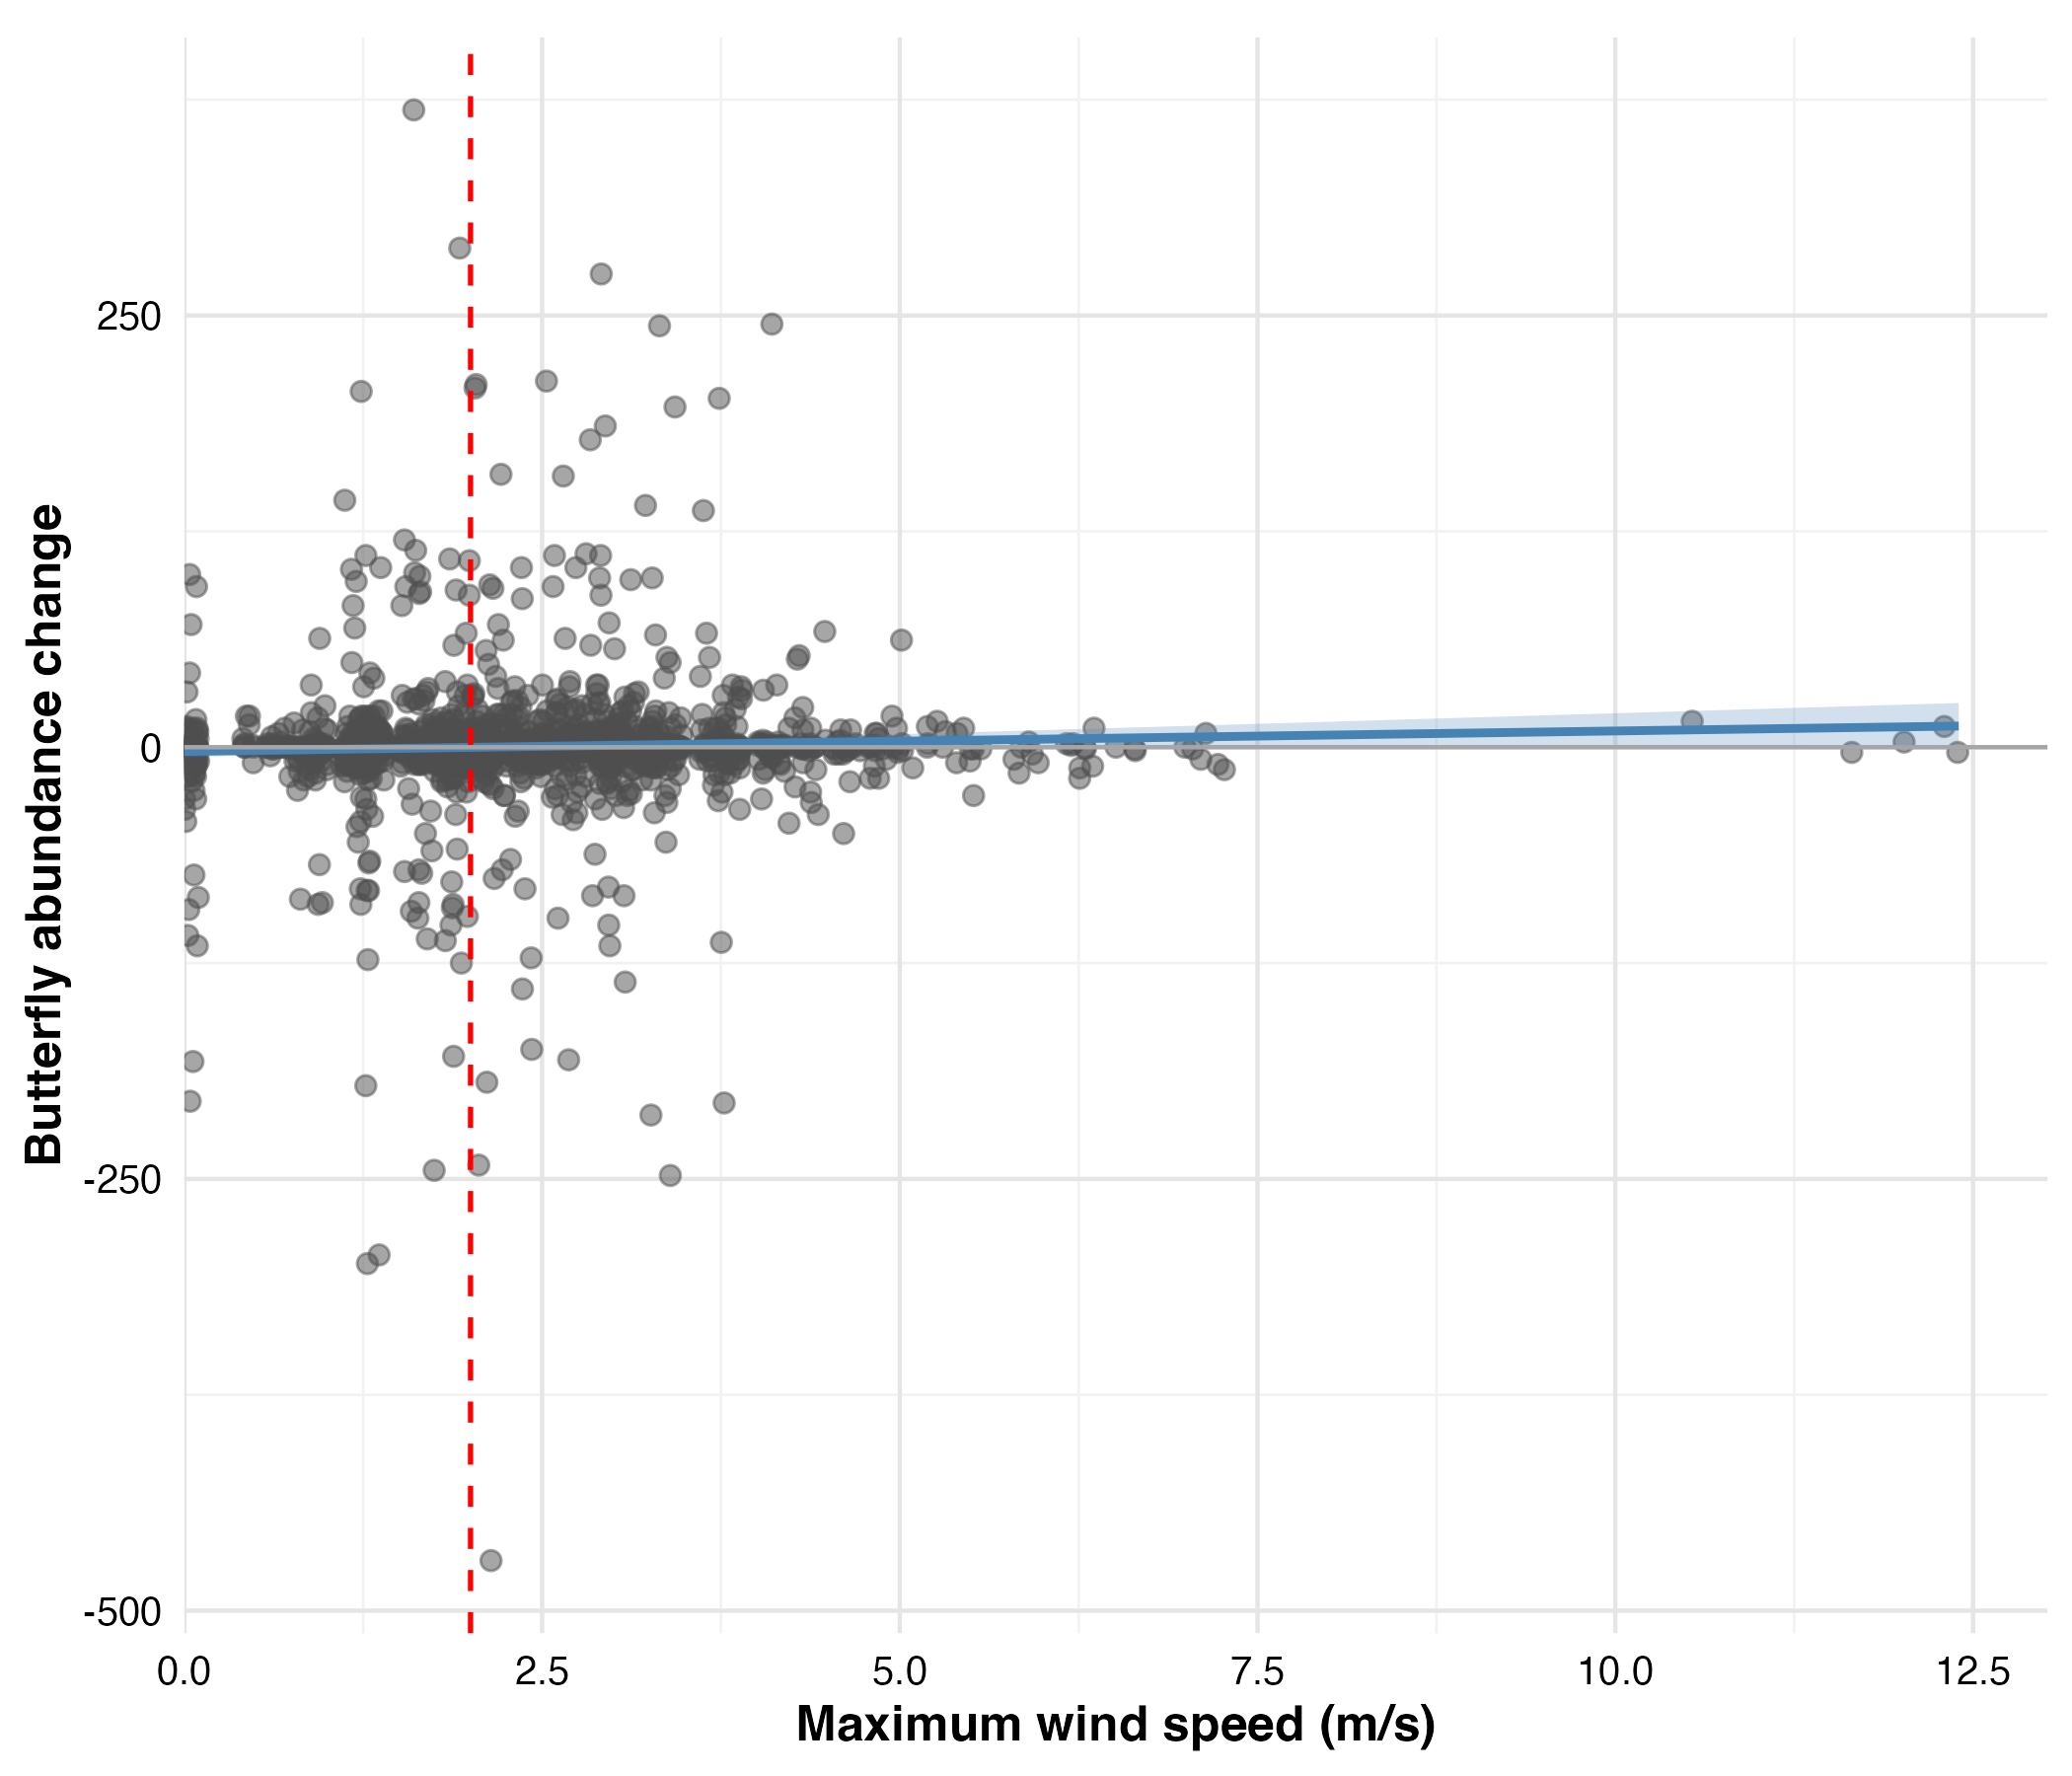
\includegraphics[width=0.8\textwidth]{supplemental/results/30_min/figures/wind_vs_change_bivariate_untransformed.png}
    \caption{Relationship between maximum wind speed and butterfly abundance change at 30-minute intervals. Each point represents a paired observation (n = 1,894). The red dashed line indicates the proposed 2 m/s behavioral threshold (r = 0.04).}
    \label{fig:wind_bivariate_30min}
\end{figure}

\begin{figure}[htbp]
    \centering
    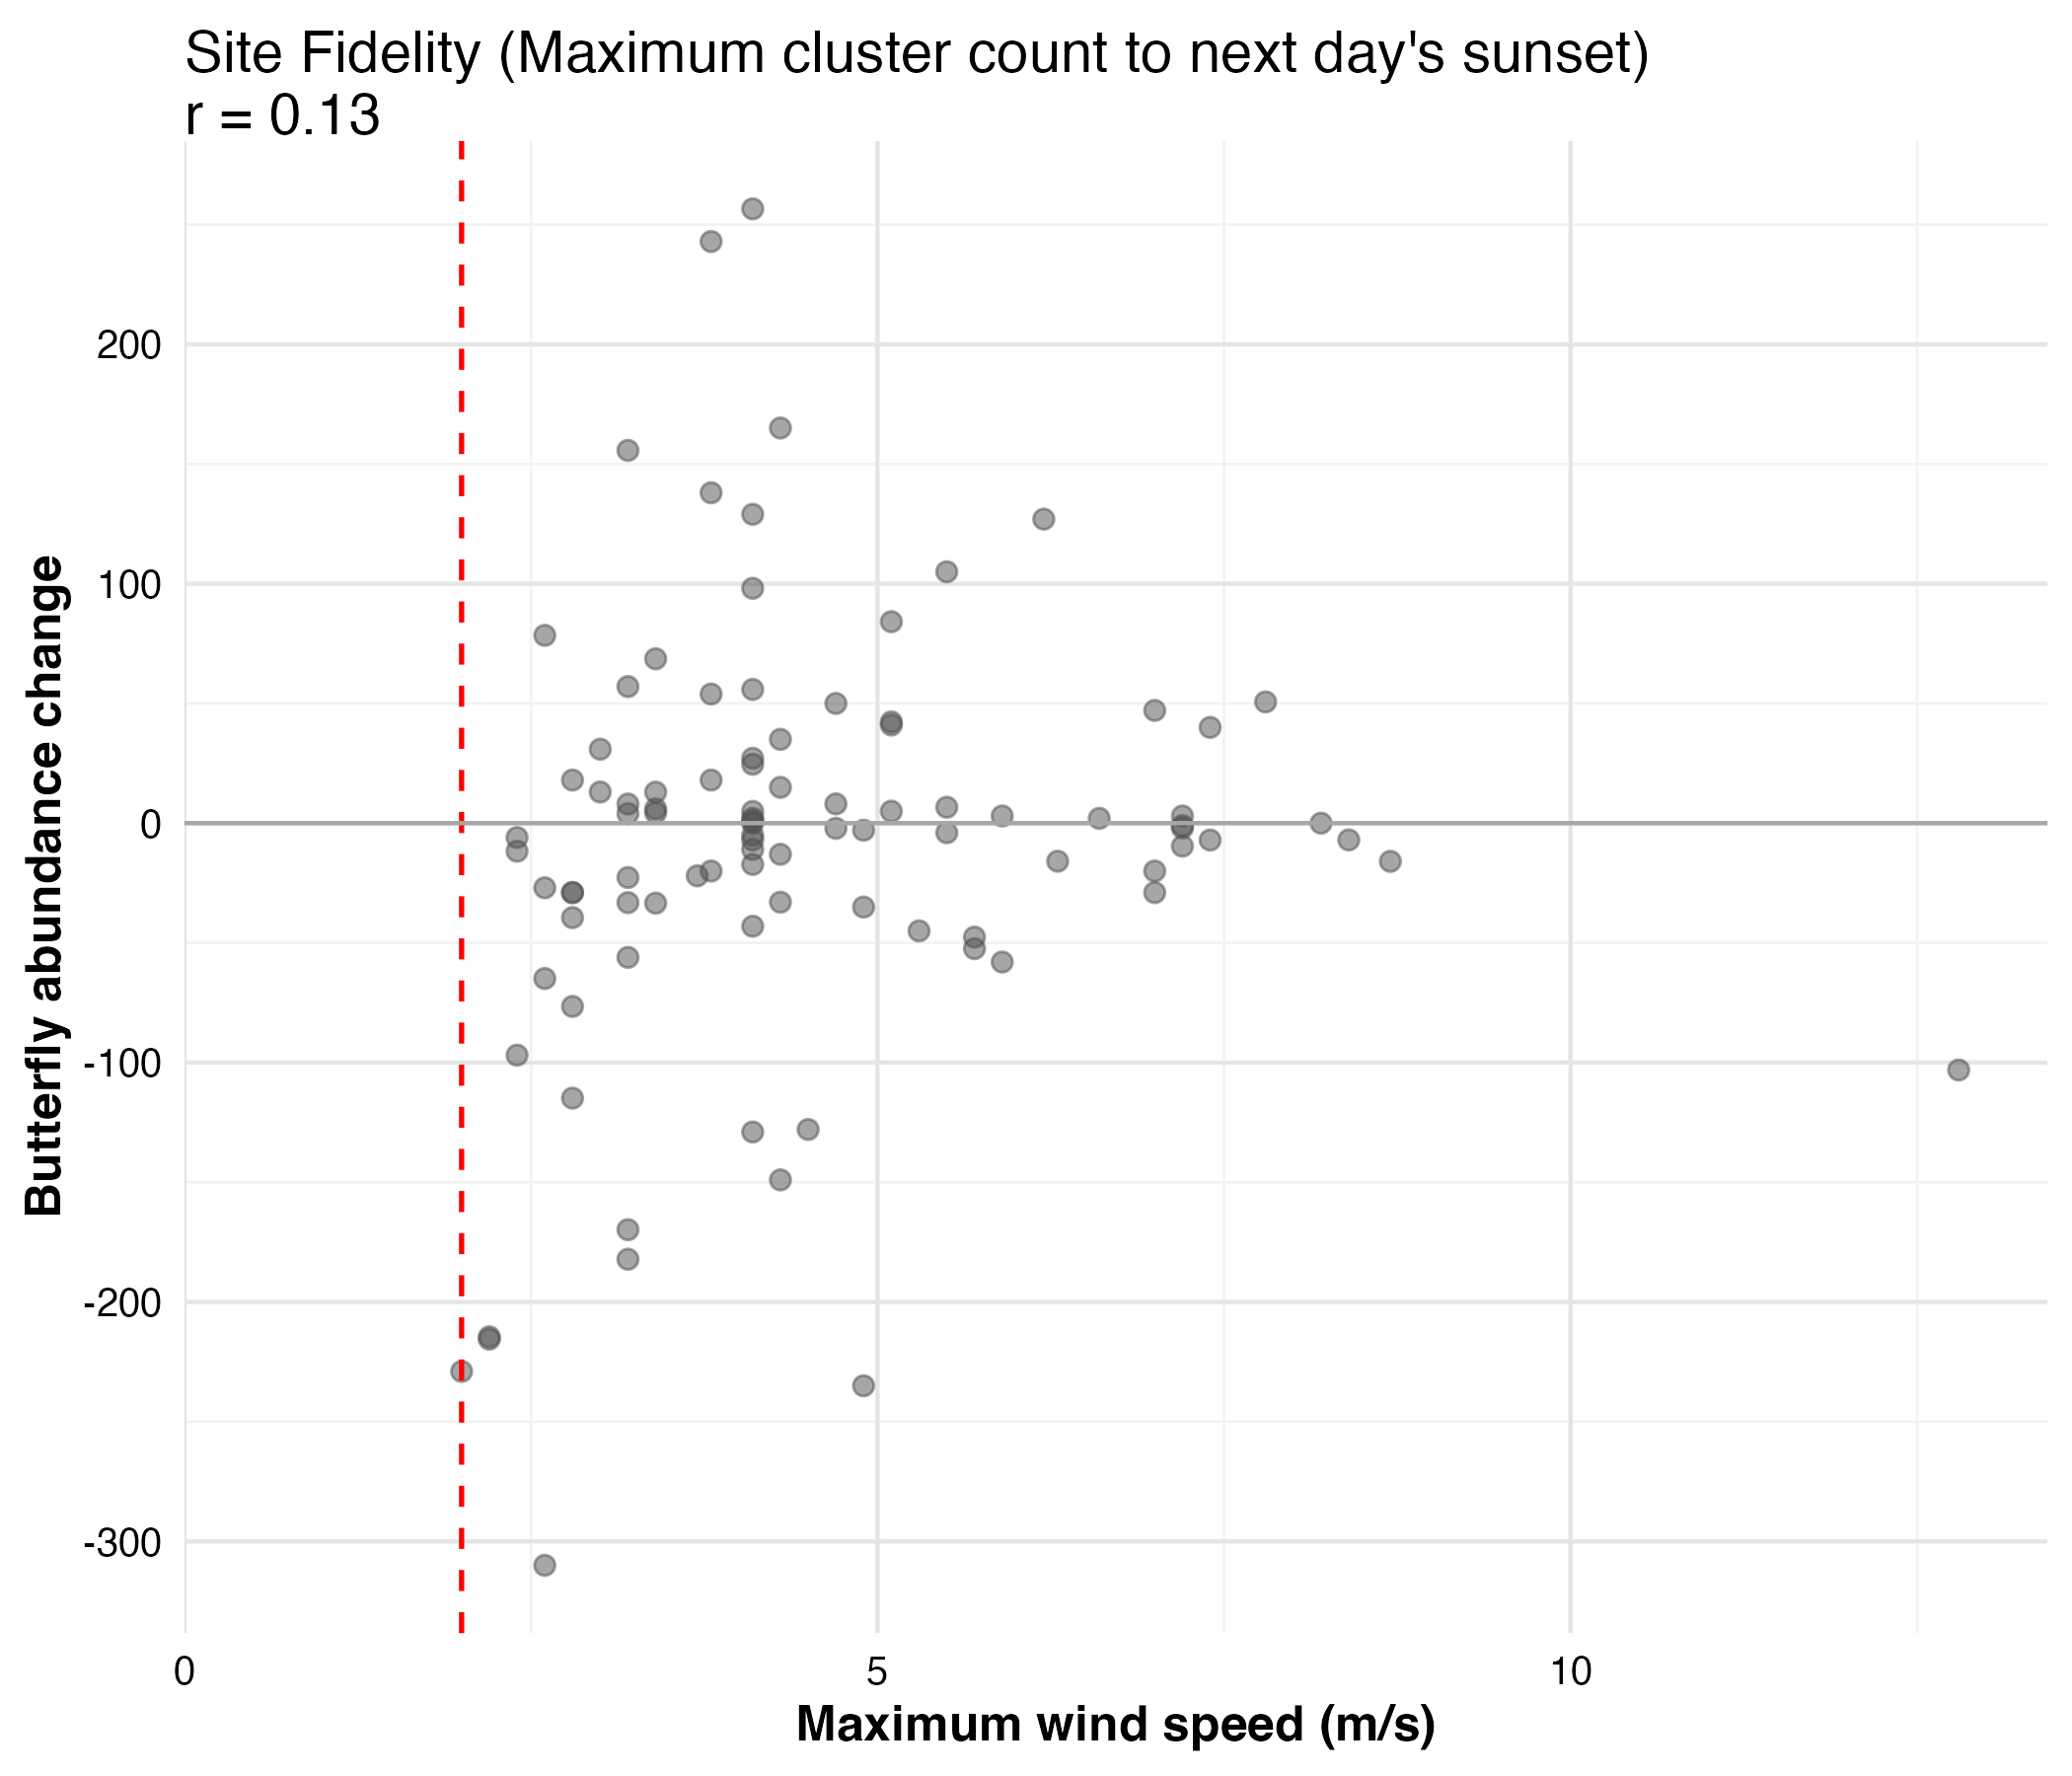
\includegraphics[width=0.8\textwidth]{supplemental/results/sunset/figures/wind_vs_change_bivariate_untransformed.png}
    \caption{Relationship between maximum wind speed and day-to-day cluster size changes from maximum count to next sunset. Each point represents consecutive day pairs at the same deployment (n = 96). The red dashed line indicates the 2 m/s threshold. All 96 observations experienced winds exceeding this threshold (r = 0.13).}
    \label{fig:wind_bivariate_sunset}
\end{figure}

\subsection{Wind Disruption Analysis}

To examine how monarchs respond to immediate environmental conditions, we analyzed 1,894 paired observations collected at 30-minute intervals throughout the overwintering season. This responsive change analysis tested whether short-term fluctuations in cluster size could be explained by concurrent weather variables, particularly wind exposure.

\subsubsection{Model Selection}

We evaluated 52 candidate models using generalized additive mixed models (GAMMs) to identify the environmental predictors of monarch abundance changes. Model selection via Akaike Information Criterion (AIC) identified M50 as the decisively best-fit model, capturing 85.8\% of the total model weight (Table~\ref{tab:export-model-selection-table}). The next best model (M23) showed substantially weaker support with $\Delta$AIC = 3.8 and only 12.6\% model weight. Model M50 incorporated smoothed terms for previous butterfly count, temperature, and time since sunrise, along with a tensor interaction between maximum wind speed and butterflies in direct sun.

\begin{table}

\caption{Top 5 models ranked by AIC (30-minute analysis)}
\centering
\begin{tabular}[t]{llrrrr}
\toprule
Model & Terms & AIC & Delta_AIC & Weight & Wind_p\\
\midrule
M50 & Previous butterfly count, Temperature, Time since sunrise, Interaction (tensor): Maximum wind speed, Butterflies in direct sun & 8074.029 & 0.000 & 0.8579 & 5.55e-05\\
M23 & Previous butterfly count, Temperature, Butterflies in direct sun, Time since sunrise & 8077.862 & 3.834 & 0.1262 & NA\\
M22 & Previous butterfly count, Temperature (linear), Butterflies in direct sun, Time since sunrise & 8082.898 & 8.869 & 0.0102 & NA\\
M24 & Previous butterfly count, Maximum wind speed, Temperature, Butterflies in direct sun, Time since sunrise & 8084.049 & 10.020 & 0.0057 & 2.18e-01\\
M52 & Temperature, Time since sunrise, Interaction (tensor): Maximum wind speed, Butterflies in direct sun & 8092.722 & 18.693 & 0.0001 & 1.13e-05\\
\bottomrule
\end{tabular}
\end{table}
 

\subsubsection{Analysis of Best Fit Model}

The best-fit model (M50) predicted change in butterfly abundance as a function of: (1) the previous 30-minute observation's butterfly count, (2) average temperature, (3) time since sunrise, and (4) an interaction between maximum wind gust speed and the number of butterflies in direct sunlight.

Statistical analysis of the model revealed significant effects for three of the four predictors (Table~\ref{tab:m50_summary}). The previous butterfly count (F = 12.50, p $<$ 0.001), time since sunrise (F = 9.85, p $<$ 0.001), and the wind-sunlight interaction (F = 4.67, p $<$ 0.001) all showed strong statistical significance. Temperature effects approached but did not reach conventional significance thresholds (F = 3.19, p = 0.057). The model explained 6.4\% of the variance in butterfly abundance changes (adjusted $R^2$ = 0.064, n = 1894).

\begin{table}[ht]
\centering
\caption{Summary of best-fit model (M50) for predicting changes in butterfly abundance. The model uses cube-root transformed butterfly count differences as the response variable.}
\label{tab:m50_summary}
\begin{tabular}{lcccc}
\toprule
\textbf{Smooth Term} & \textbf{edf} & \textbf{Ref.df} & \textbf{F} & \textbf{p-value} \\
\midrule
Previous butterfly count & 2.41 & 2.41 & 12.50 & $<$ 0.001*** \\
Average temperature & 3.68 & 3.68 & 3.19 & 0.057 \\
Time since sunrise & 4.87 & 4.87 & 9.85 & $<$ 0.001*** \\
Wind gust × Sunlight exposure & 7.35 & 7.35 & 4.67 & $<$ 0.001*** \\
\midrule
\multicolumn{5}{l}{\textit{Model performance:} Adj. $R^2$ = 0.064, Scale est. = 4.03, n = 1894} \\
\bottomrule
\end{tabular}
\end{table}

Partial effects for the smooth terms are shown in Figure~\ref{fig:partial_effects_30min}. The previous butterfly count showed a significant non-linear negative relationship (p < 0.001) consistent with proportionally greater departures from larger aggregations. Time since sunrise captured a significant diurnal pattern (p < 0.001) with morning departures and afternoon returns. Temperature showed a marginally non-significant trend (p = 0.057) suggesting possible effects near the 12.7–16°C flight threshold range.

\begin{figure}[htbp]
    \centering
    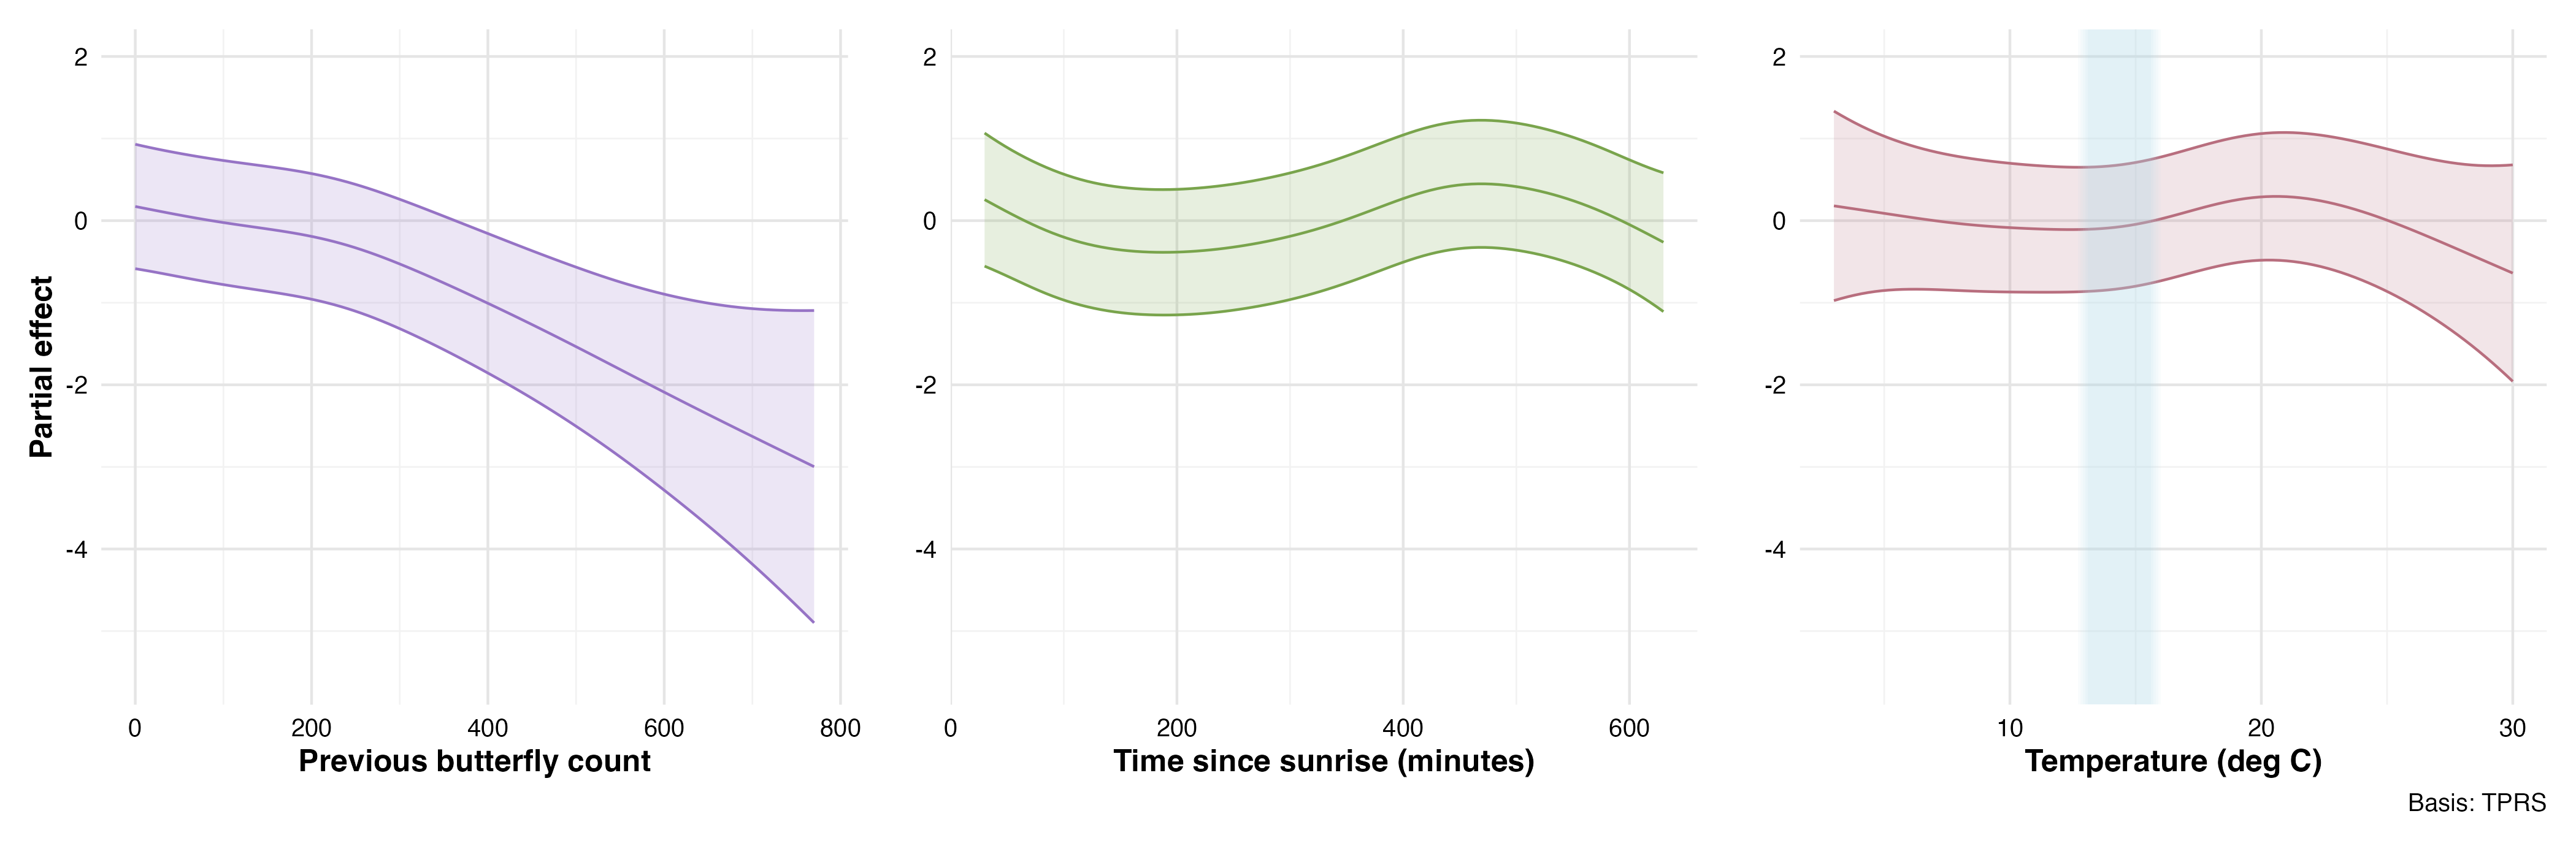
\includegraphics[width=\textwidth]{supplemental/results/30_min/figures/partial_effects_best_1x3.png}
    \caption{Partial effects of environmental predictors on monarch butterfly abundance changes from the best-fit GAMM model (M50). Shaded regions represent 95\% confidence intervals.}
    \label{fig:partial_effects_30min}
\end{figure}

The tensor interaction between wind speed and butterflies in direct sun (p < 0.001) revealed a complex conditional relationship where wind effects depended on solar exposure conditions (Figure~\ref{fig:interaction_wind_sun}). When butterflies in direct sun were held at zero (all butterflies in indirect light), cluster size changes showed no consistent trend across the observed wind speed range (0-12 m/s). Conversely, when wind was held constant, low numbers of butterflies in direct sun were associated with decreasing cluster sizes across the time window, while higher counts led to increasing cluster sizes across the time window. At low butterfly counts in direct sun, the wind effect showed distinct patterns: clusters decreased in size at very calm winds (<1 m/s), showed no change from 1-3 m/s, and tended to increase from 4-8 m/s. At moderate wind speeds (1-3 m/s) and high butterfly counts (>100), cluster sizes tended to decrease. However, as wind speeds exceeded 3 m/s at these same butterfly counts, the pattern reversed, with cluster sizes increasing. The red dashed line at 2 m/s indicates the behavioral threshold identified in previous analyses. Gray regions mask areas too distant from observed data points for reliable interpretation, and caution is warranted when interpreting the strongest partial effects at the edges of the data distribution, where observations are sparse and interpolation artifacts may occur. Notably, the overwhelming majority of observations occurred at very low butterfly counts in direct sun, emphasizing that most clustering behavior happens when few butterflies are exposed to direct sunlight. 

\begin{figure}[htbp]
    \centering
    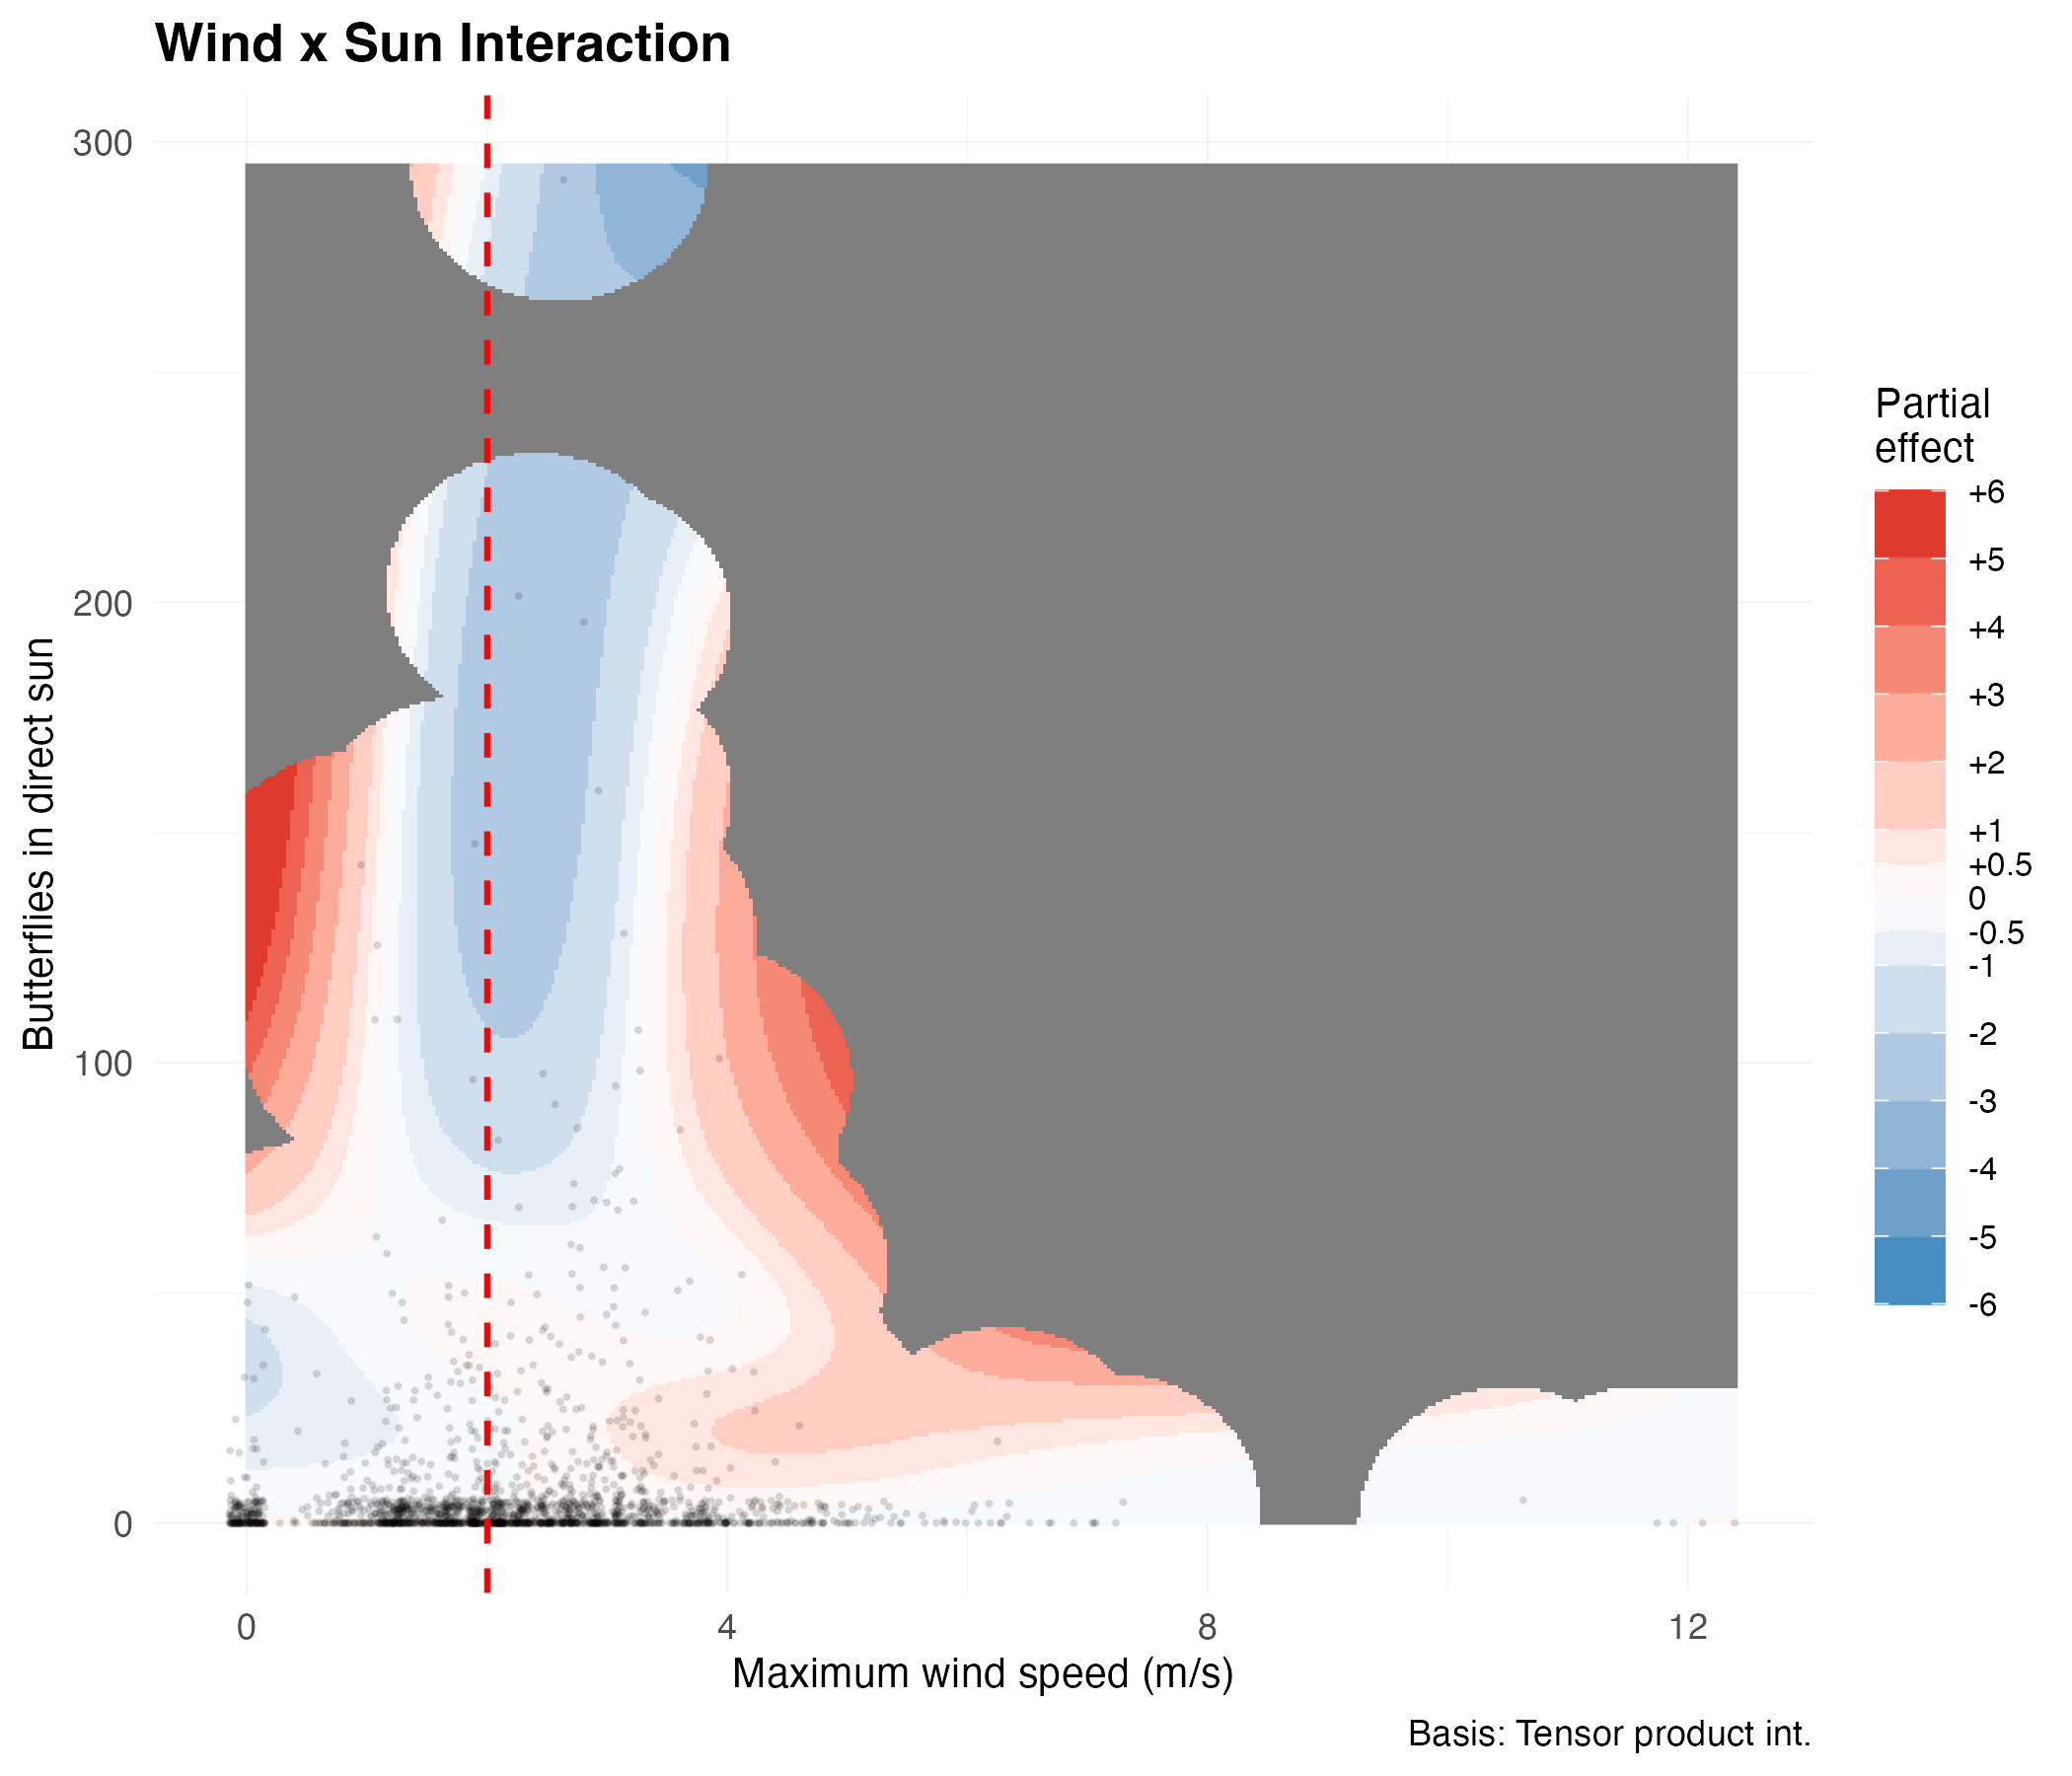
\includegraphics[width=0.8\textwidth]{supplemental/results/30_min/figures/interaction_wind_x_sun_binned.png}
    \caption{Figure 1.3 Tensor smooth interaction between maximum wind speed (m/s) and butterflies in direct sun on cluster size changes. Color gradient indicates partial effect magnitude (red = positive, blue = negative). Black points show observed data distribution. Red dashed line marks the 2 m/s behavioral threshold. Gray regions indicate areas beyond reliable interpolation range.}
    \label{fig:interaction_wind_sun}
\end{figure}

\subsubsection{Model Diagnostics}

Model diagnostic plots confirmed the adequacy of the GAMM specification (Figure~\ref{fig:model_diagnostics_30min}). Residual versus fitted value plots showed no systematic patterns or heteroscedasticity, indicating appropriate model structure. The quantile-quantile plot revealed approximately normal residual distribution with minor deviations in the tails, acceptable given the large sample size and complexity of ecological data.

\begin{figure}[htbp]
    \centering
    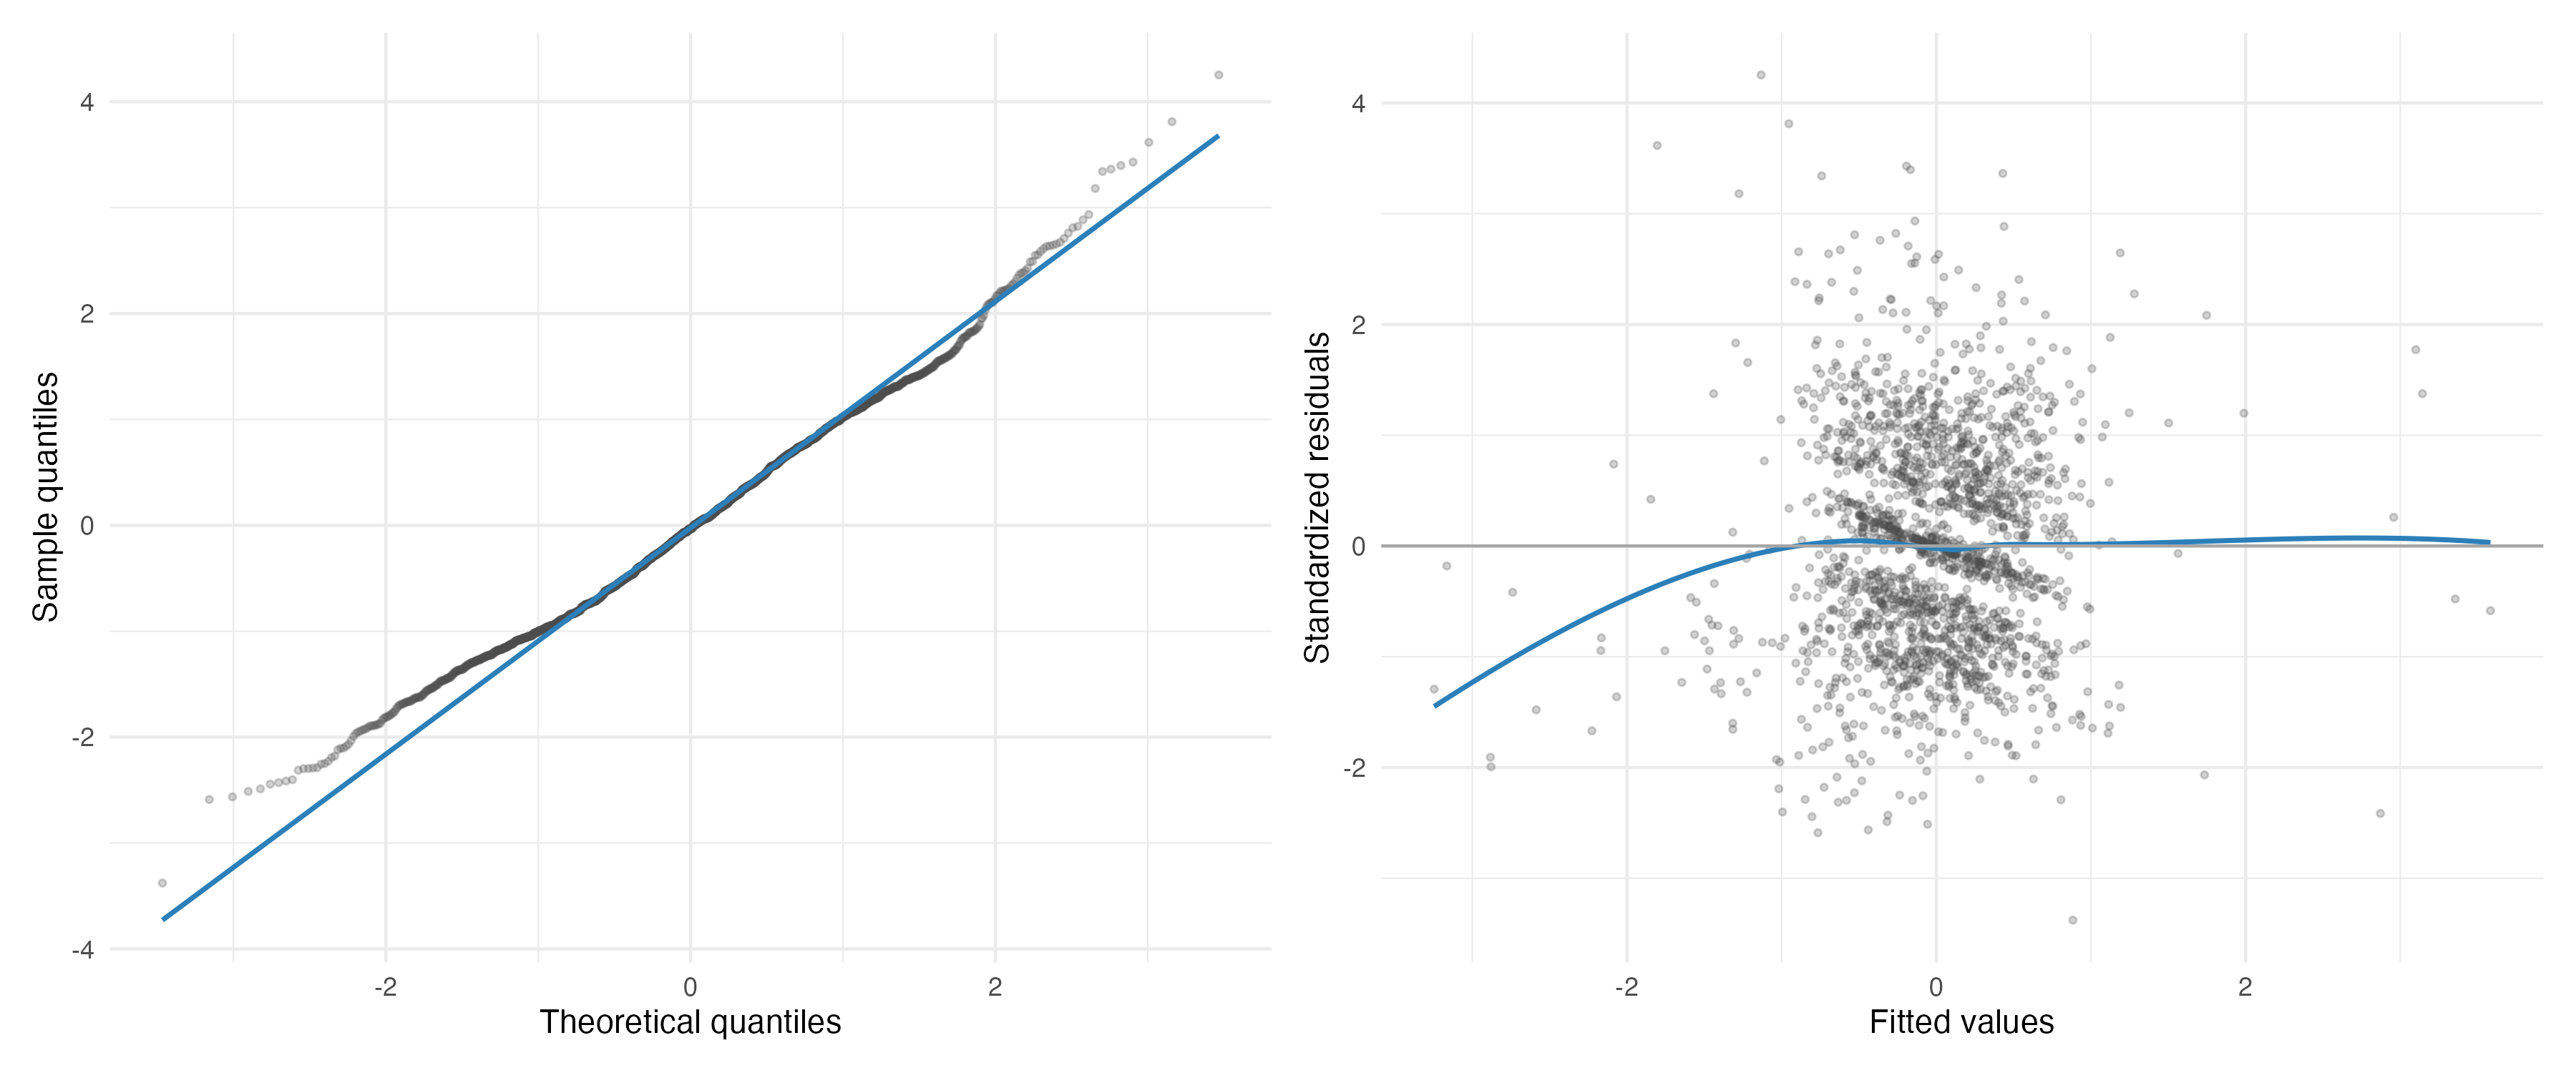
\includegraphics[width=0.9\textwidth]{supplemental/results/30_min/figures/diag_qq_and_residuals_1x2.png}
    \caption{Diagnostic plots for the best-fit GAMM model (M50). Left panel shows quantile-quantile plot comparing model residuals to theoretical normal distribution. Right panel displays residuals versus fitted values to assess homoscedasticity and model adequacy.}
    \label{fig:model_diagnostics_30min}
\end{figure}

Basis dimension checks confirmed adequate smoothing parameter selection for all model terms (Table~\ref{tab:gam_basis_check}). All smooth functions showed k-index values near 1.0, indicating sufficient basis dimensions to capture the underlying functional forms. None of the smooth terms showed evidence of undersmoothing (all p-values > 0.05), with the possible exception of time within day which showed marginal evidence (k-index = 0.96, p = 0.065). These diagnostics confirm that the chosen basis dimensions adequately represent the complexity of the smooth relationships without overfitting.

\begin{table}[htbp]
\centering
\caption[Basis dimension adequacy checks (M50)]{Basis dimension adequacy checks for smooth terms in best-fit GAMM model (M50). Low p-values (k-index < 1) may indicate insufficient basis dimensions, particularly when edf approaches k'.}
\label{tab:gam_basis_check}
\begin{tabular}{lrrrc}
\toprule
Smooth Term & k' & edf & k-index & p-value \\
\midrule
s(total butterflies $t_{lag}$) & 9.00 & 2.41 & 1.00 & 0.735 \\
s(temperature avg) & 9.00 & 3.67 & 1.02 & 0.895 \\
s(time within day $t$) & 9.00 & 4.87 & 0.96 & 0.065 \\
ti(max gust, butterflies direct sun $t_{lag}$) & 16.00 & 7.35 & 0.99 & 0.490 \\
\bottomrule
\end{tabular}
\end{table}


Temporal autocorrelation analysis revealed minimal residual correlation structure after accounting for the AR(1) correlation within deployment days (Figure~\ref{fig:acf_diagnostics}). The autocorrelation function showed rapid decay with all lags beyond lag 1 falling within the significance bounds, confirming that the model adequately captured temporal dependencies in the data. This indicates that our mixed-effects structure with autoregressive errors appropriately addressed the repeated measures nature of the time-series observations.

\begin{figure}[htbp]
    \centering
    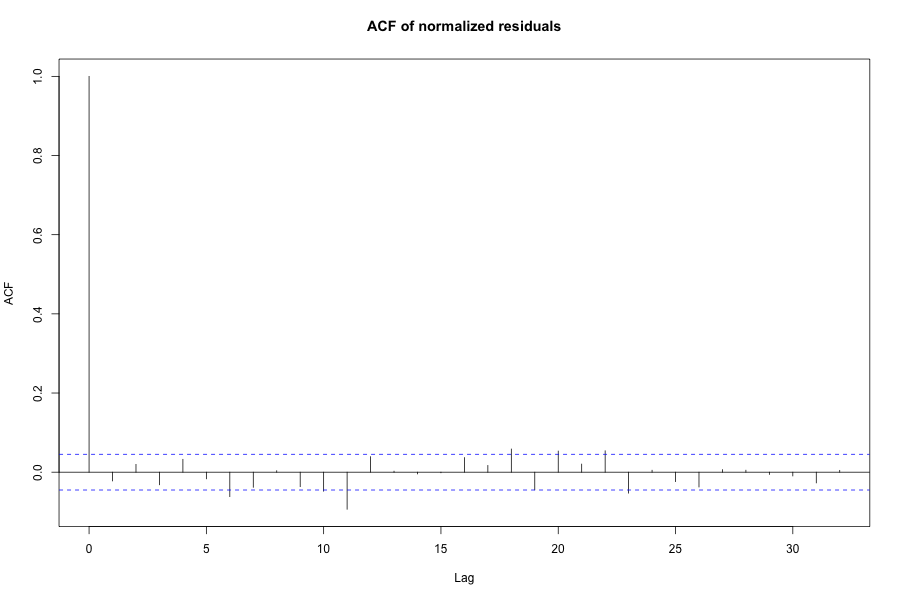
\includegraphics[width=0.8\textwidth]{supplemental/results/30_min/figures/diag_acf.png}
    \caption{Autocorrelation function of model residuals showing minimal temporal correlation after accounting for AR(1) structure within deployment days. Blue dashed lines indicate 95\% confidence bounds for white noise.}
    \label{fig:acf_diagnostics}
\end{figure} 

\subsubsection{Threshold Wind Disruption Analysis}

We conducted this threshold analysis to determine whether wind is best characterized as a continuous variable or a binary disruption threshold, regardless of whether it operates independently or conditionally on other factors. To test the hypothesis that wind acts as a binary disruption threshold rather than a continuous variable, we repeated the entire analysis using minutes above 2 m/s as the wind predictor. This threshold-based approach directly tests our second hypothesis that wind becomes disruptive above the 2 m/s threshold, which, if it represents a meaningful biological boundary, should predict declining monarch abundance at roosts experiencing sustained winds exceeding this threshold. The best threshold model (T50) maintained the same structure as our primary analysis but showed notably weaker performance (Table~\ref{tab:threshold_model_selection}).

While T50 achieved the lowest AIC among threshold models, it failed to decisively outperform simpler alternatives, capturing only 55.4\% of model weight compared to 40.4\% for the model without any wind term (T23). The negligible difference in AIC ($\Delta$AIC = 0.63) between these models indicates substantial certainty that the threshold wind variable does not substantially improve predictions. Despite this weaker overall performance (adjusted $R^2$ = 0.061 compared to 0.064 in the primary analysis), the interaction term between minutes above threshold and butterflies in direct sun achieved statistical significance (p = 0.0001), and notably, T50 was the only model among the top five candidates to include any wind parameters. This suggests that while the threshold approach may not optimally characterize wind effects, the interaction with solar exposure warrants examination.

\begin{table}

\caption{\label{tab:threshold_model_selection}Top 5 models ranked by AIC (30-minute threshold analysis)}
\centering
\begin{tabular}[t]{llrrr}
\toprule
Model & Terms & AIC & $\Delta$AIC & Weight\\
\midrule
T50 & Previous butterfly count, Temperature, Time since sunrise, Interaction (tensor): Minutes above 2 m/s, Butterflies in direct sun & 8077.23 & 0.00 & 0.55\\
T23 & Previous butterfly count, Temperature, Butterflies in direct sun, Time since sunrise & 8077.86 & 0.63 & 0.40\\
T22 & Previous butterfly count, Temperature (linear), Butterflies in direct sun, Time since sunrise & 8082.90 & 5.67 & 0.03\\
T24 & Previous butterfly count, Minutes above 2 m/s, Temperature, Butterflies in direct sun, Time since sunrise & 8085.41 & 8.18 & 0.01\\
T47 & Temperature, Butterflies in direct sun, Time since sunrise & 8097.30 & 20.07 & 0.00\\
\bottomrule
\end{tabular}
\end{table}


The interaction partial effects plot from the threshold analysis reveals complex conditional relationships between wind exposure duration and solar conditions (Figure~\ref{fig:threshold_interaction}). When butterflies in direct sun are held at zero (all butterflies in indirect light), cluster size changes show no apparent trend across the entire range of wind exposure duration, from no time above threshold to the full 30-minute observation period. This suggests that wind effects on shaded butterflies are minimal regardless of exposure duration.

As butterfly counts in direct sun increase, distinct patterns emerge. At moderate counts (25-50 butterflies), cluster sizes tend to decrease when wind exposure extends from 15 to 25 minutes above threshold. However, at the extremes of sustained wind exposure (greater than 25 minutes), cluster sizes tend to increase. When wind exposure is minimal (0-5 minutes above threshold), increasing butterfly counts in sun show no effect on cluster size changes. The strongest effects appear at intermediate wind exposure durations (15-25 minutes) combined with moderate solar exposure levels.

The same caveats apply regarding sparse data at the extremes and the limits of interpolation, particularly given that most observations occurred at low butterfly counts in direct sun.

\begin{figure}[htbp]
    \centering
    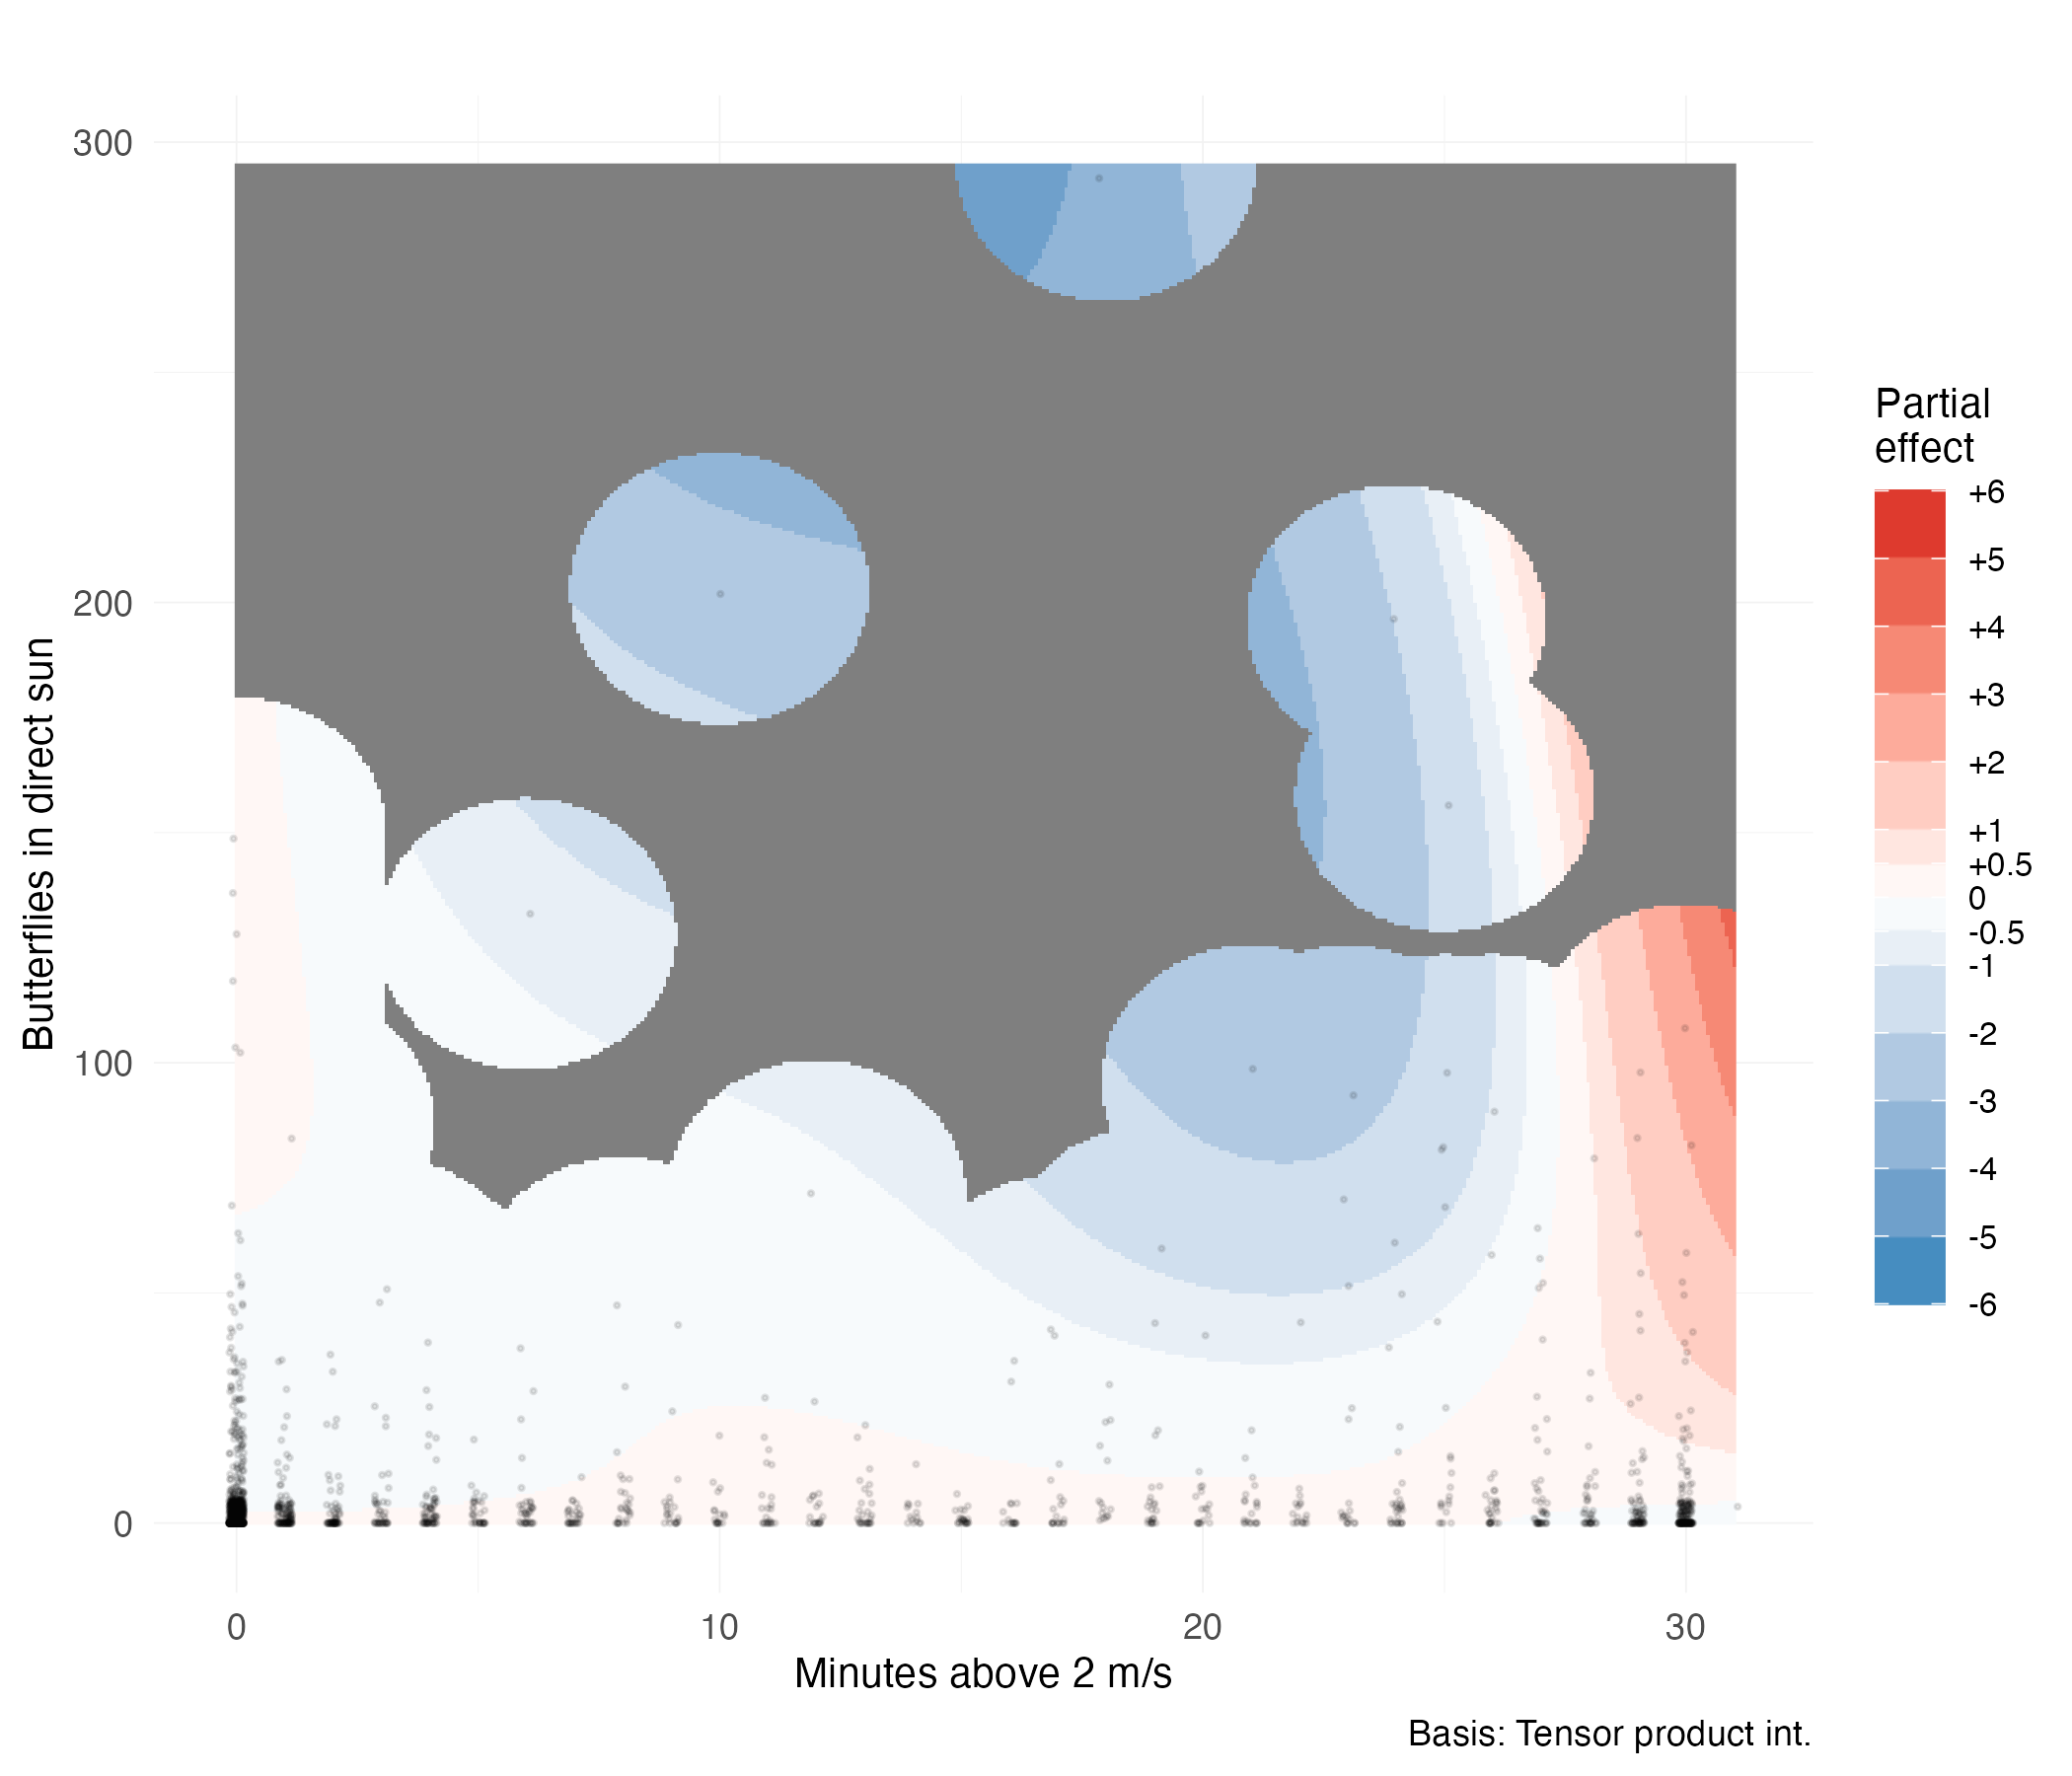
\includegraphics[width=0.8\textwidth]{supplemental/results/30_min_threshold/figures/interaction_wind_x_sun_binned.png}
    \caption{Tensor smooth interaction between minutes above 2 m/s wind threshold and butterflies in direct sun on cluster size changes. Color gradient indicates partial effect magnitude (red = positive, blue = negative). Black points show observed data distribution. Gray regions indicate areas beyond reliable interpolation range.}
    \label{fig:threshold_interaction}
\end{figure} 

\subsection{Statistical Power to Detect Wind Effects}

Post-hoc power analysis confirmed our study had adequate statistical power to detect biologically meaningful wind effects (Table~\ref{tab:power_analysis}). With 1,894 paired observations, we achieved 87.5\% power to detect moderate effect sizes (0.15 standard deviations) and 98.5\% power to detect larger effects (0.20 standard deviations). Power for small effects (0.10 standard deviations) was 56\%, while very small effects (0.05 standard deviations) yielded only 16.5\% power. These results indicate that our study has sufficient statistical power for effect sizes of biological relevance.

\begin{table}[htbp]
\centering
\caption[Statistical power to detect wind effects]{Estimated power to detect wind effects of varying magnitudes. Effect sizes are expressed in standard deviations of the response variable (cube root transformed change in butterfly abundance).}
\label{tab:power_analysis}
\begin{tabular}[t]{lrrl}
\toprule
  & Effect Size (SD units) & Power (Proportion) & Power (\%)\\
\midrule
0.05 & 0.05 & 0.165 & 16.5\%\\
0.1 & 0.10 & 0.560 & 56\%\\
0.15 & 0.15 & 0.875 & 87.5\%\\
0.2 & 0.20 & 0.985 & 98.5\%\\
\bottomrule
\end{tabular}
\end{table}


\subsection{Site Fidelity Analysis}

The preceding wind disruption analysis examined how monarchs respond to immediate environmental conditions, testing whether strong wind events trigger the rapid cluster departures predicted by the behavioral disruption hypothesis. While our 30-minute analysis revealed no simple relationship between wind speed and cluster changes, it assumed butterflies could respond instantaneously to unfavorable conditions. This assumption may not hold when adverse conditions occur during periods when temperatures fall below the flight threshold, constraining monarchs' ability to relocate until environmental conditions permit flight. Furthermore, monarchs may make clustering decisions on longer temporal horizons than our 30-minute observation intervals capture. To address these limitations, we conducted a complementary analysis examining day-to-day roost dynamics by tracking clusters from one day's maximum count through the following day's sunset, when darkness precludes further aggregation changes. This approach tests whether cumulative weather exposure over extended periods influences site fidelity decisions, with substantial decreases in cluster size indicating reduced site suitability and potential roost abandonment, while stable or increasing counts suggest the site remains suitable despite weather exposure.

To implement this day-to-day analysis, we examined 96 consecutive-day pairs from the same deployment dataset using biologically-aligned temporal windows. The primary analysis employed a sunset window spanning from the previous day's maximum count to the current day's last observation (mean duration = 29.6 hours), capturing the full period from peak aggregation through the subsequent roosting decision. A secondary analysis using fixed 24-hour windows (n = 94 pairs) provided a sensitivity test of our findings.

Daily maximum cluster sizes ranged from 0 to 770 butterflies (mean = 134.7 ± 138.1), with day-to-day changes in maximum count ranging from losses of 376 butterflies to gains of 464 butterflies (mean change = -10.5 ± 111.6). Within the sunset windows, maximum wind gusts ranged from 2.0 to 12.8 m/s (mean = 4.5 ± 1.8 m/s), with all observation windows exceeding the proposed 2 m/s threshold. Cumulative direct sun exposure varied from 0 to 1,122 butterfly-observations in sunlight per window (mean = 139.8 ± 206.9), reflecting diverse thermal exposure conditions across monitoring days.

\subsubsection{Model Selection}

We evaluated 76 candidate models using generalized additive mixed models (GAMMs) to identify environmental predictors of day-to-day changes in maximum cluster size. The model space included null, single-predictor, interaction-only, additive, main effects with interactions, and complex formulations, all incorporating deployment random intercepts and AR(1) temporal correlation. Model selection via corrected Akaike Information Criterion (AICc) identified The best fit Model (M32) as the decisively best-fit model, capturing 84.7\% of the total model weight (Table~\ref{tab:sunset-model-selection-table}). The next best model (M52) showed substantially weaker support with $\Delta$AICc = 5.6 and only 5.2\% model weight. Model M32 incorporated a tensor smooth interaction between maximum wind gust and cumulative direct sun exposure, along with baseline controls for previous day's maximum count and window duration.

\begin{table}

\caption{Top 5 models ranked by AICc (sunset analysis)}
\centering
\begin{tabular}[t]{llrrr}
\toprule
Model & Terms & AICc & $\Delta$AICc & Weight\\
\midrule
M32 & Interaction (tensor): Maximum wind gust, Cumulative butterflies in direct sun & 648.85 & 0.00 & 0.85\\
M52 & Maximum wind gust, Cumulative butterflies in direct sun, Interaction (tensor): Maximum wind gust, Cumulative butterflies in direct sun & 654.45 & 5.60 & 0.05\\
M20 & Interaction (tensor): Minimum temperature, Cumulative butterflies in direct sun & 656.77 & 7.92 & 0.02\\
M46 & Maximum temperature, Cumulative butterflies in direct sun, Interaction (tensor): Maximum temperature, Cumulative butterflies in direct sun & 657.70 & 8.85 & 0.01\\
M30 & Interaction (tensor): Temperature at previous maximum count, Cumulative butterflies in direct sun & 657.90 & 9.06 & 0.01\\
\bottomrule
\end{tabular}
\end{table}


\subsubsection{Analysis of Best Fit Model}

The best-fit model (M32) predicted square-root transformed change in butterfly abundance as a function of: (1) the previous day's maximum butterfly count, (2) window duration in hours, and (3) a tensor smooth interaction between maximum wind gust speed and cumulative butterflies in direct sunlight.

Statistical analysis revealed significant effects for the previous day's maximum count (t = -4.988, p < 0.001) and the wind-sunlight interaction (F = 4.097, p < 0.001), while window duration showed no significant effect (t = -1.067, p = 0.289) (Table~\ref{tab:m32_summary}). The model explained 39.7\% of the variance in day-to-day cluster size changes (adjusted $R^2$ = 0.397, n = 96), representing substantially greater explanatory power than the 30-minute responsive change analysis.

\begin{table}[ht]
\centering
\caption[Summary of best-fit model (M32)]{Summary of best-fit model (M32) for predicting site fidelity. The model uses square-root transformed day-to-day changes in butterfly count as the response variable.}
\label{tab:m32_summary}
\begin{tabular}{lcccc}
\toprule
\textbf{Smooth Term} & \textbf{edf} & \textbf{Ref.df} & \textbf{F} & \textbf{p-value} \\
\midrule
Previous day maximum count & 1.00 & 1.00 & 24.88 & $<$ 0.001*** \\
Window duration & 1.00 & 1.00 & 1.14 & 0.289 \\
Wind gust × Sunlight exposure & 6.68 & 6.68 & 4.10 & $<$ 0.001*** \\
\midrule
\multicolumn{5}{l}{\textit{Model performance:} Adj. $R^2$ = 0.397, Scale est. = 41.06, n = 96} \\
\bottomrule
\end{tabular}
\end{table}

The previous day's maximum count showed a significant negative linear relationship (coefficient = -0.030, SE = 0.006), indicating that larger clusters experienced proportionally greater losses between days. This pattern aligns with the wind disruption analysis. Window duration showed no significant relationship with cluster size changes. Partial effects for these linear predictors are shown in Figure~\ref{fig:partial_effects_sunset}.

\begin{figure}[htbp]
    \centering
    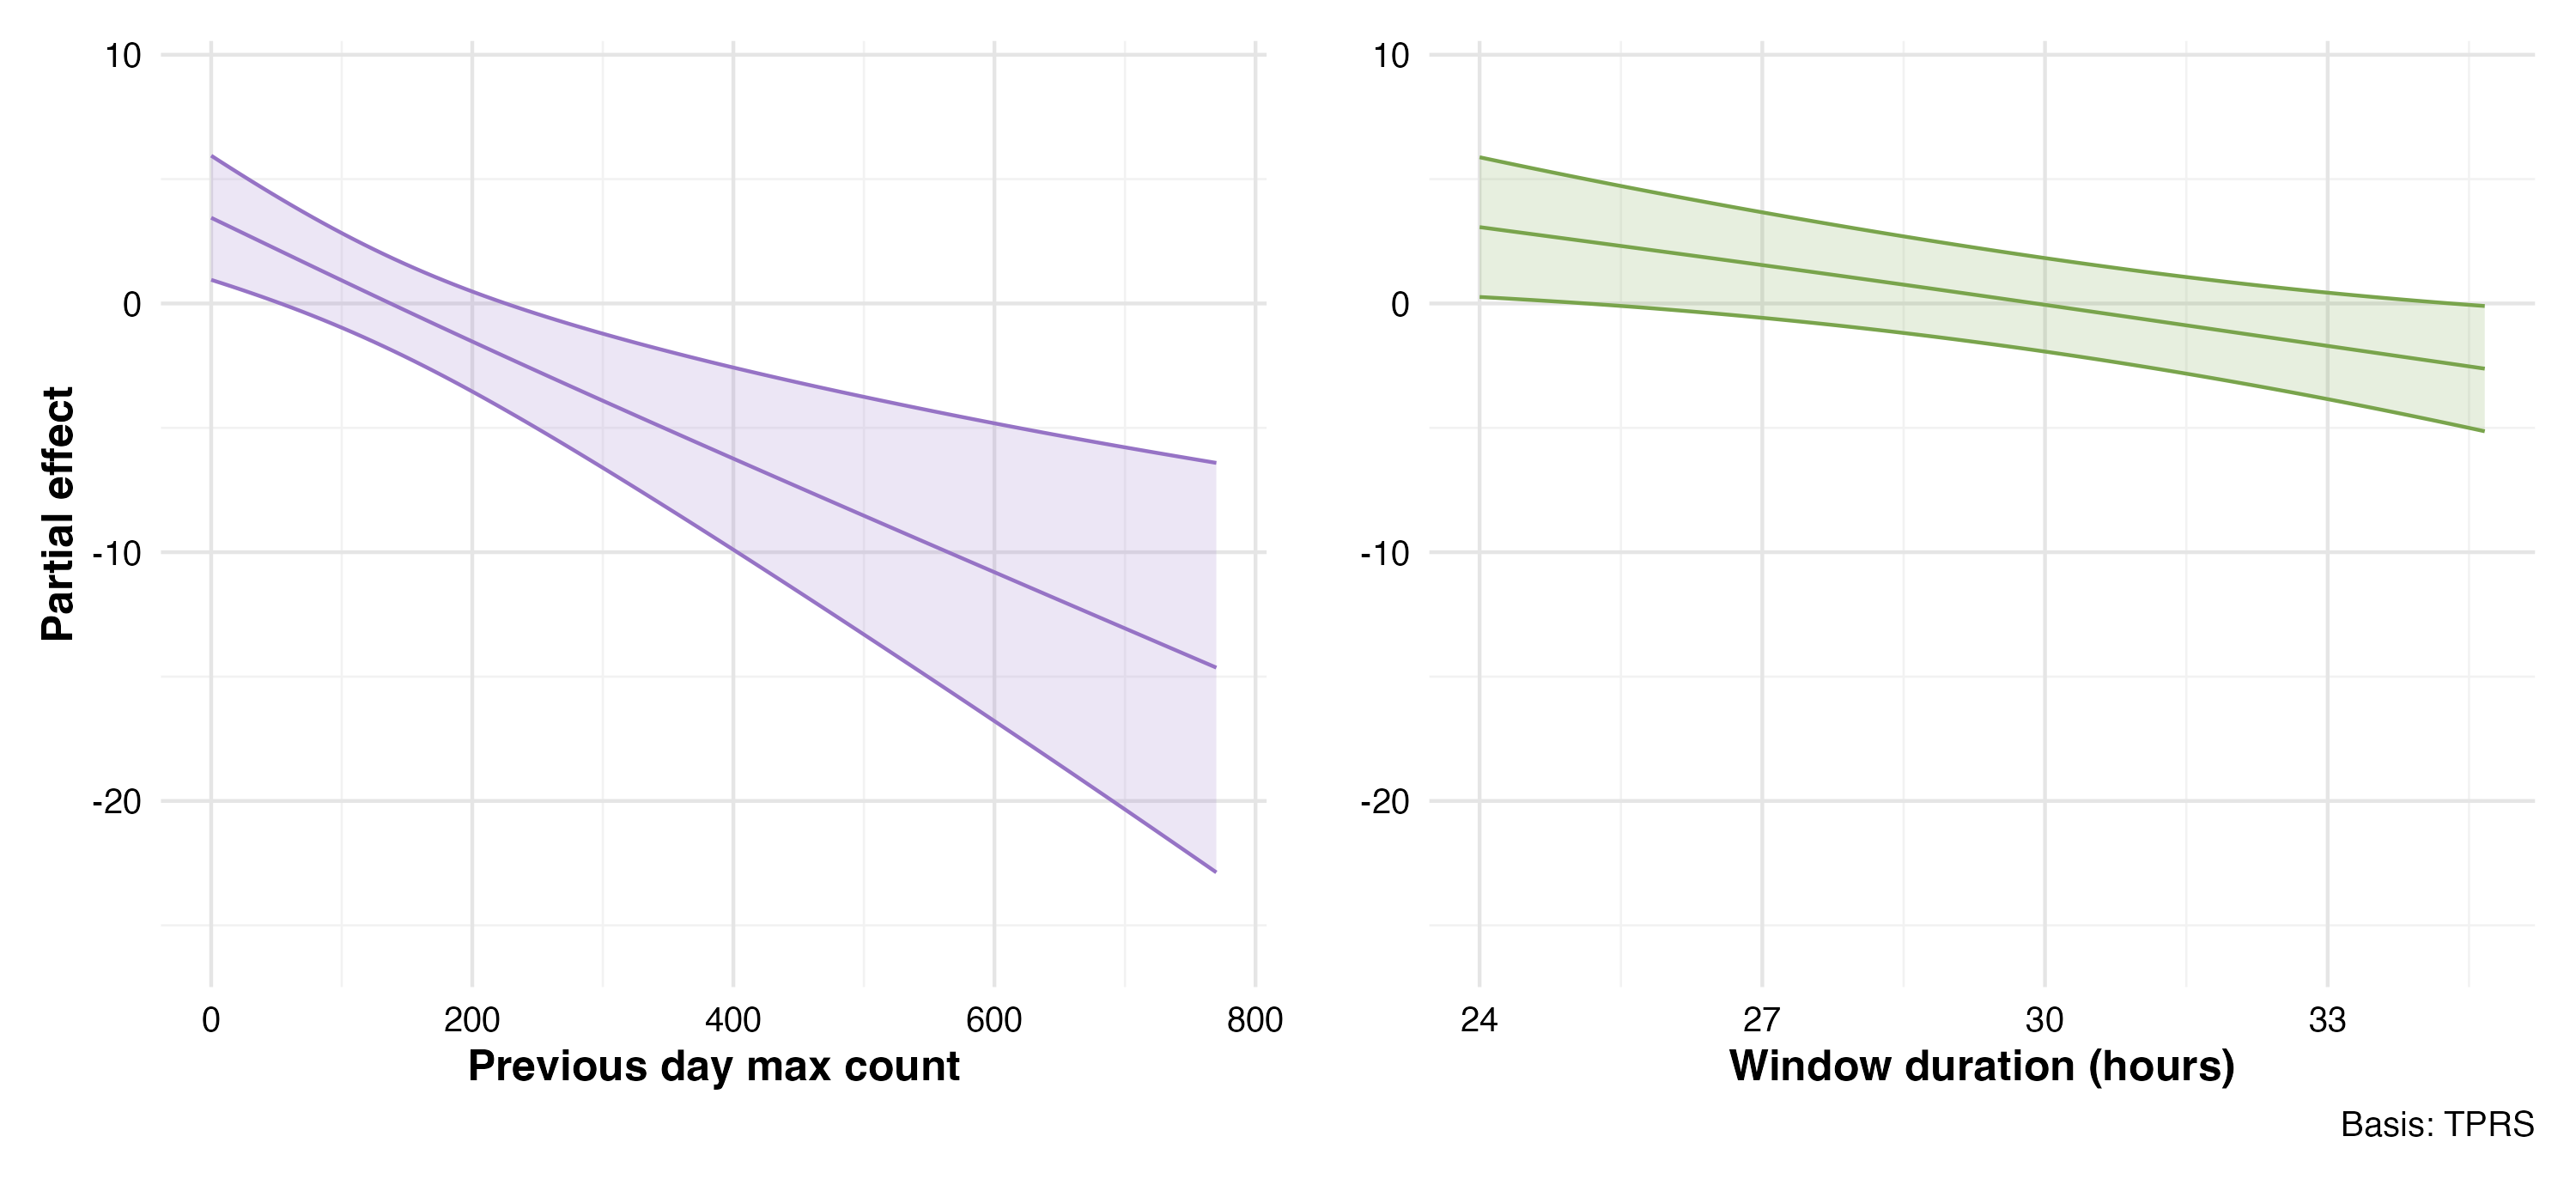
\includegraphics[width=\textwidth]{supplemental/results/sunset/figures/partial_effects_best_1x2.png}
    \caption{Partial effects of control variables on day-to-day monarch butterfly cluster size changes from the best-fit GAMM model (M32). Left panel shows the strong negative effect of previous day maximum count. Right panel shows window duration had no significant effect on cluster size changes. Shaded regions represent 95\% confidence intervals.}
    \label{fig:partial_effects_sunset}
\end{figure}

The tensor smooth interaction between maximum wind gust and cumulative direct sun exposure (p < 0.001) revealed complex conditional relationships between sustained weather exposure and cumulative butterflies in direct light (Figure~\ref{fig:interaction_wind_sun_sunset}). All observations during the study period experienced wind speeds exceeding 2 m/s. Under low wind speeds around 2 m/s with minimal butterfly counts in direct sun, clusters increased the following day, though this pattern reversed sharply as butterfly counts increased, resulting in decreased cluster sizes. When butterfly counts approached zero, cluster sizes showed minimal change to slight decreases across most wind speeds, with the exception of extreme wind values where sparse data limits interpretation. At intermediate to high values of both wind speed and butterfly sun exposure, cluster sizes increased the next day. Interpretation requires caution at interpolation boundaries and regions with single observations. 

\begin{figure}[htbp]
    \centering
    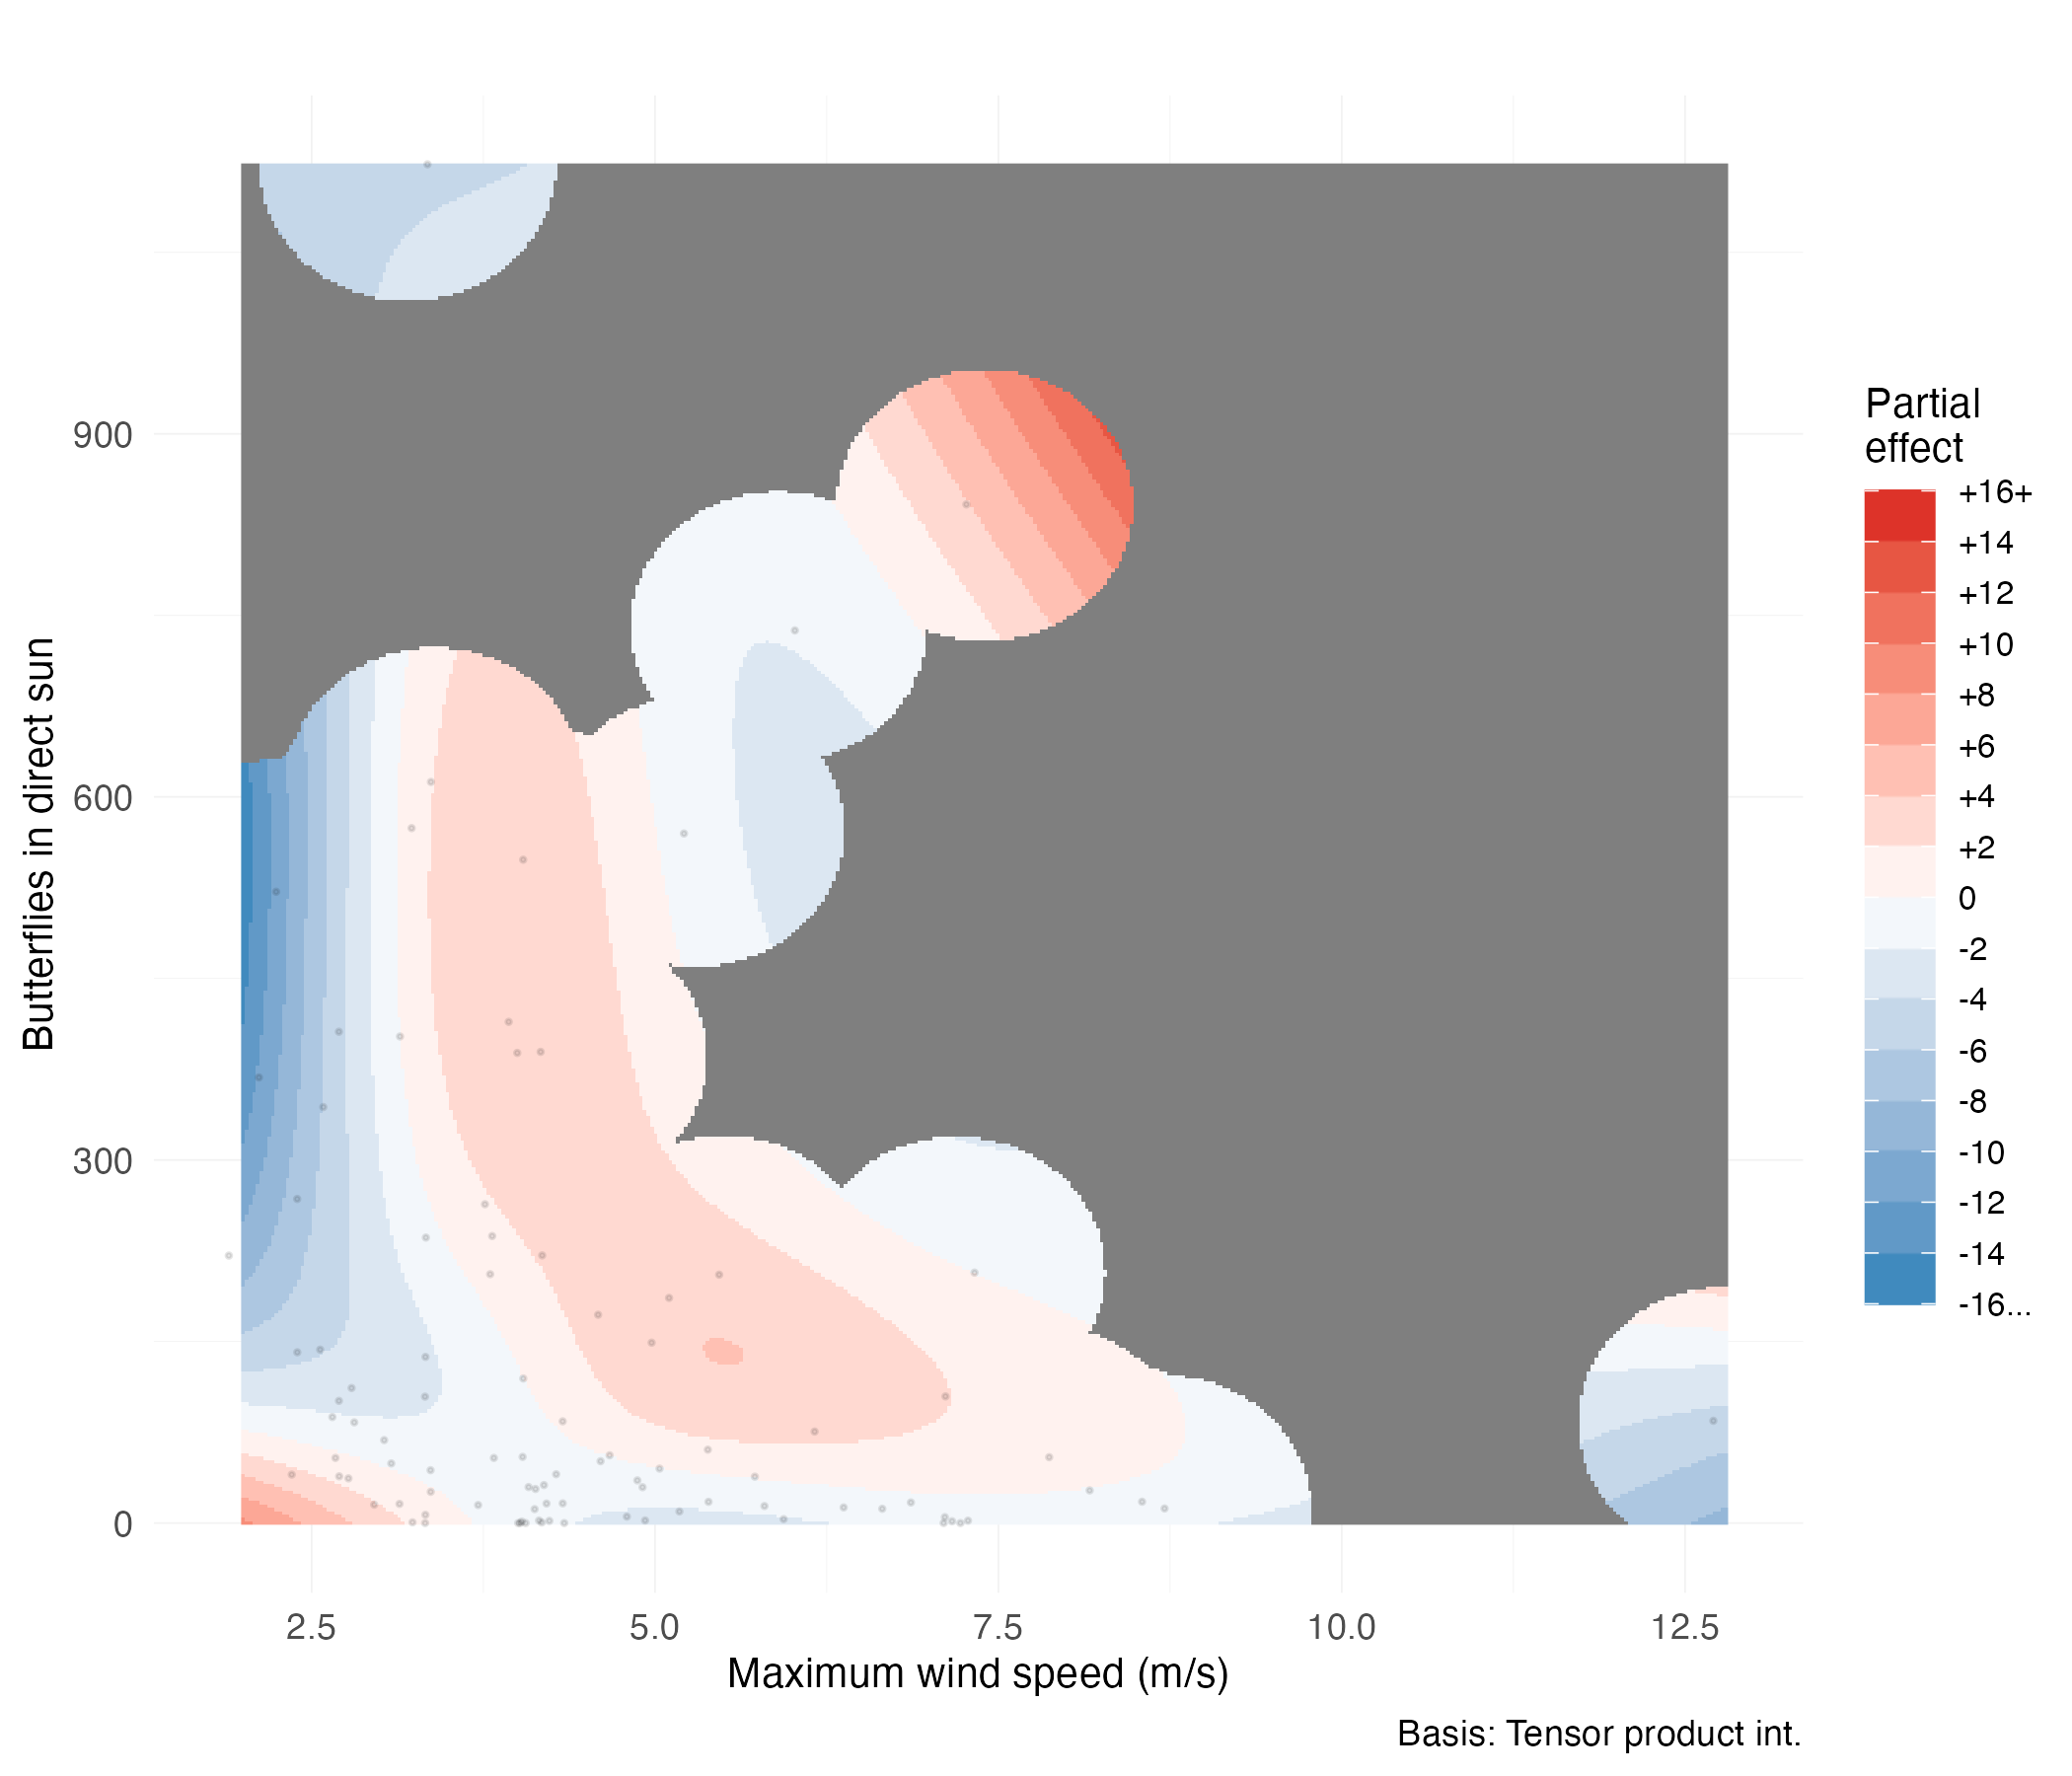
\includegraphics[width=0.8\textwidth]{supplemental/results/sunset/figures/interaction_wind_x_sun_binned.png}
    \caption{Tensor smooth interaction between maximum wind gust (m/s) and cumulative butterflies in direct sun on day-to-day cluster size changes. Color gradient indicates partial effect magnitude on square-root transformed scale (red = positive, blue = negative). Black points show observed data distribution. Gray regions indicate areas beyond reliable interpolation range.}
    \label{fig:interaction_wind_sun_sunset}
\end{figure}

\subsubsection{Model Diagnostics}

Model diagnostic plots confirmed the adequacy of the GAMM specification (Figure~\ref{fig:model_diagnostics_sunset}). Residual versus fitted value plots showed no systematic patterns or heteroscedasticity, indicating appropriate model structure. The quantile-quantile plot revealed approximately normal residual distribution with minor deviations in the tails, acceptable given the sample size and complexity of ecological data.

\begin{figure}[htbp]
    \centering
    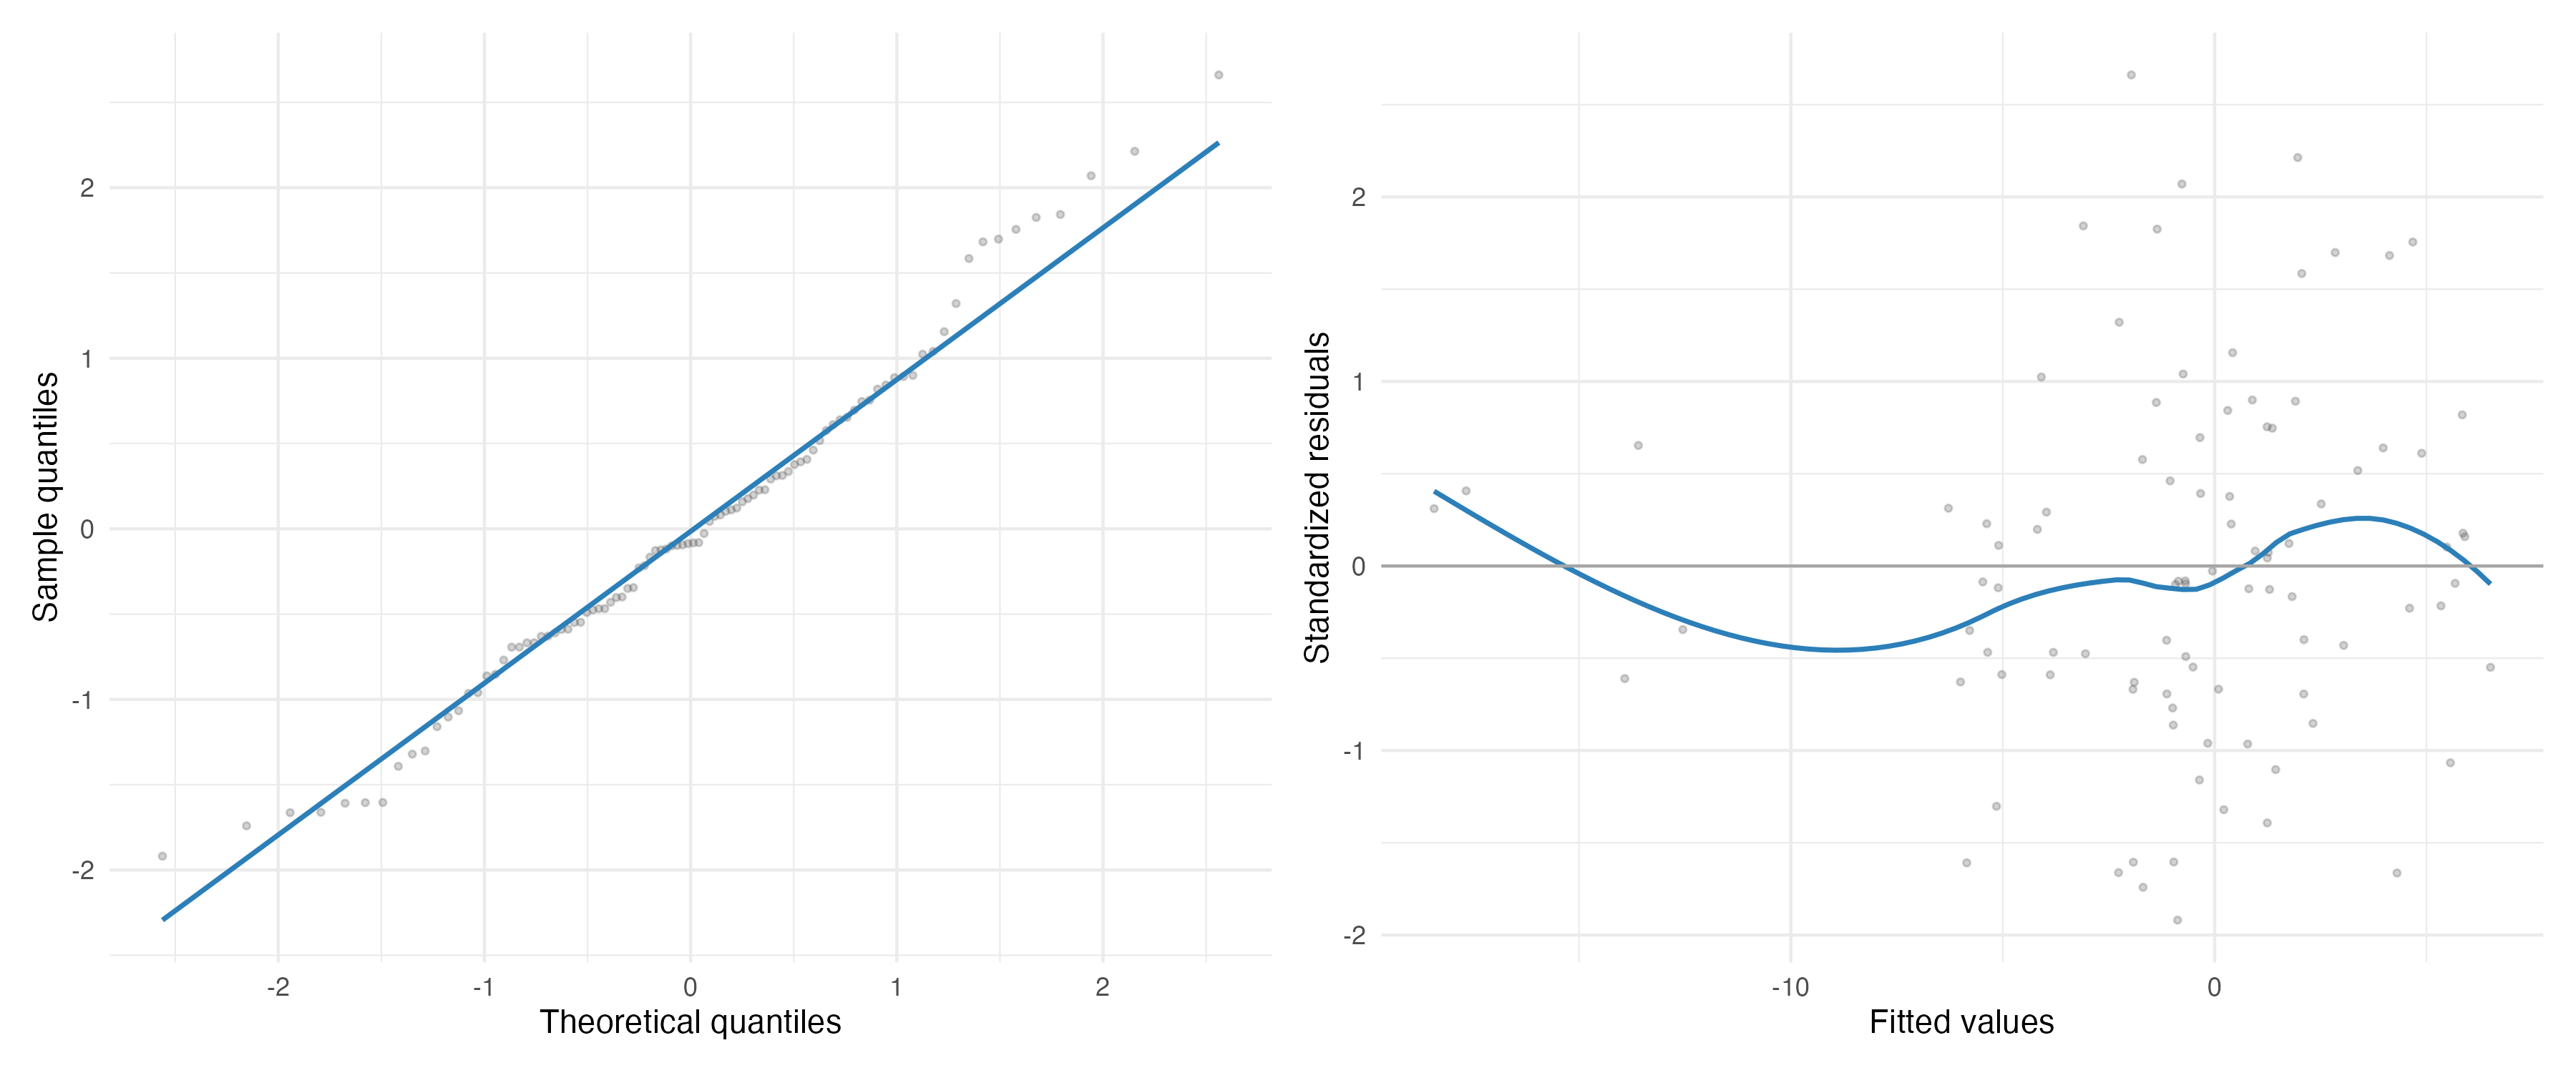
\includegraphics[width=0.9\textwidth]{supplemental/results/sunset/figures/diag_qq_and_residuals_1x2.png}
    \caption{Diagnostic plots for the best-fit GAMM model (M32). Left panel shows quantile-quantile plot comparing model residuals to theoretical normal distribution. Right panel displays residuals versus fitted values to assess homoscedasticity and model adequacy.}
    \label{fig:model_diagnostics_sunset}
\end{figure}

Basis dimension checks confirmed adequate smoothing parameter selection for the tensor smooth interaction term. The wind-sunlight interaction showed a k-index value of 1.06 (p = 0.72), indicating sufficient basis dimensions to capture the underlying functional form without evidence of undersmoothing. This confirms that the chosen basis dimensions adequately represent the complexity of the smooth relationship without overfitting.

Temporal autocorrelation analysis revealed minimal residual correlation structure after accounting for the AR(1) correlation within deployment days (Figure~\ref{fig:acf_diagnostics_sunset}). The autocorrelation function showed rapid decay with all lags beyond lag 1 falling within the significance bounds, confirming that the model adequately captured temporal dependencies in the data. 

\begin{figure}[htbp]
    \centering
    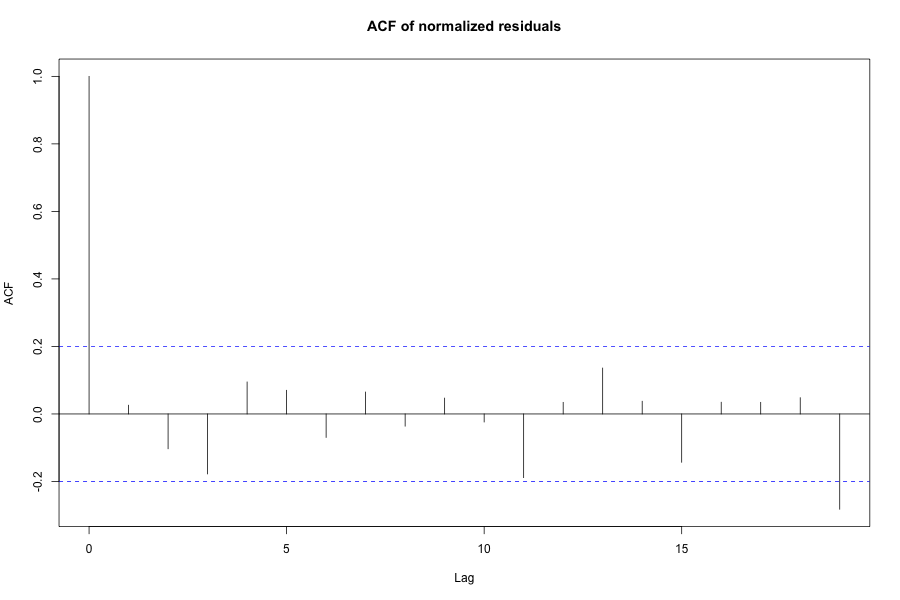
\includegraphics[width=0.8\textwidth]{supplemental/results/sunset/figures/diag_acf.png}
    \caption{Autocorrelation function of model residuals showing minimal temporal correlation after accounting for AR(1) structure within deployment days. Blue dashed lines indicate 95\% confidence bounds for white noise.}
    \label{fig:acf_diagnostics_sunset}
\end{figure}

\subsection{Robustness Analysis: 24-Hour Butterfly Change}

To assess the robustness of our findings, we conducted an analysis examining butterfly cluster changes over 24-hour periods rather than sunset-specific intervals. This analysis evaluated the same 72 candidate models using identical GAMM specifications with deployment random intercepts and AR(1) temporal correlation (adjusted R2 of 0.061 to 0.064). Notably, model selection converged on the same structural form as the primary sunset analysis. Model M31, incorporating a tensor smooth interaction between maximum wind gust and cumulative direct sun exposure, emerged as the decisively best-fit model with 50.7\% of the total model weight (Table~\ref{tab:24hr-model-selection-table}). Alternative models showed substantially weaker support, with the next best model achieving only 8.4\% weight and $\Delta$AICc = 3.6.

\begin{table}[htbp]
\centering
\caption[Top models from 24-hour robustness analysis]{Top five models from 24-hour robustness analysis ranked by AICc. The best-fit model (M31) included a tensor smooth interaction between maximum wind gust and cumulative butterflies in direct sun, matching the structure identified in the sunset-specific analysis but applied to 24-hour periods.}
\label{tab:24hr-model-selection-table}
\begin{tabularx}{\textwidth}{lXcccc}
\toprule
Model & Description & AICc & $\Delta$AICc & Weight & adj. $R^2$ \\
\midrule
M31 & Wind $\times$ sun exposure (smooth) & 636.3 & 0.0 & 0.507 & 0.235 \\
M23 & Temperature $\times$ wind (smooth) & 639.9 & 3.6 & 0.084 & -- \\
M29 & Temperature $\times$ sun exposure (smooth) & 640.8 & 4.4 & 0.056 & -- \\
M19 & Min. temp. $\times$ sun exposure (smooth) & 641.1 & 4.8 & 0.047 & -- \\
M51 & Wind + sun + wind$\times$sun (smooth) & 641.7 & 5.4 & 0.034 & -- \\
\bottomrule
\end{tabularx}
\end{table}

The 24-hour analysis revealed qualitatively similar interaction patterns to the sunset-specific model, though with attenuated effect magnitudes reflecting the longer temporal window (Figure~\ref{fig:interaction_wind_sun_24hr}). Under low wind conditions (approximately 2 m/s) with minimal butterflies in direct sun, clusters increased over the subsequent 24 hours. This effect reversed sharply as butterfly counts in direct sun increased under low winds, resulting in rapid cluster size decreases. When no butterflies occupied direct sun positions, cluster sizes remained relatively stable across wind speed values. Intermediate values for both wind speed and sun exposure produced cluster size increases. The convergent model selection and consistent interaction patterns across temporal scales strengthen confidence in the identified environmental relationships, while interpretation requires similar caution near data boundaries and regions with sparse observations.

\begin{figure}[htbp]
    \centering
    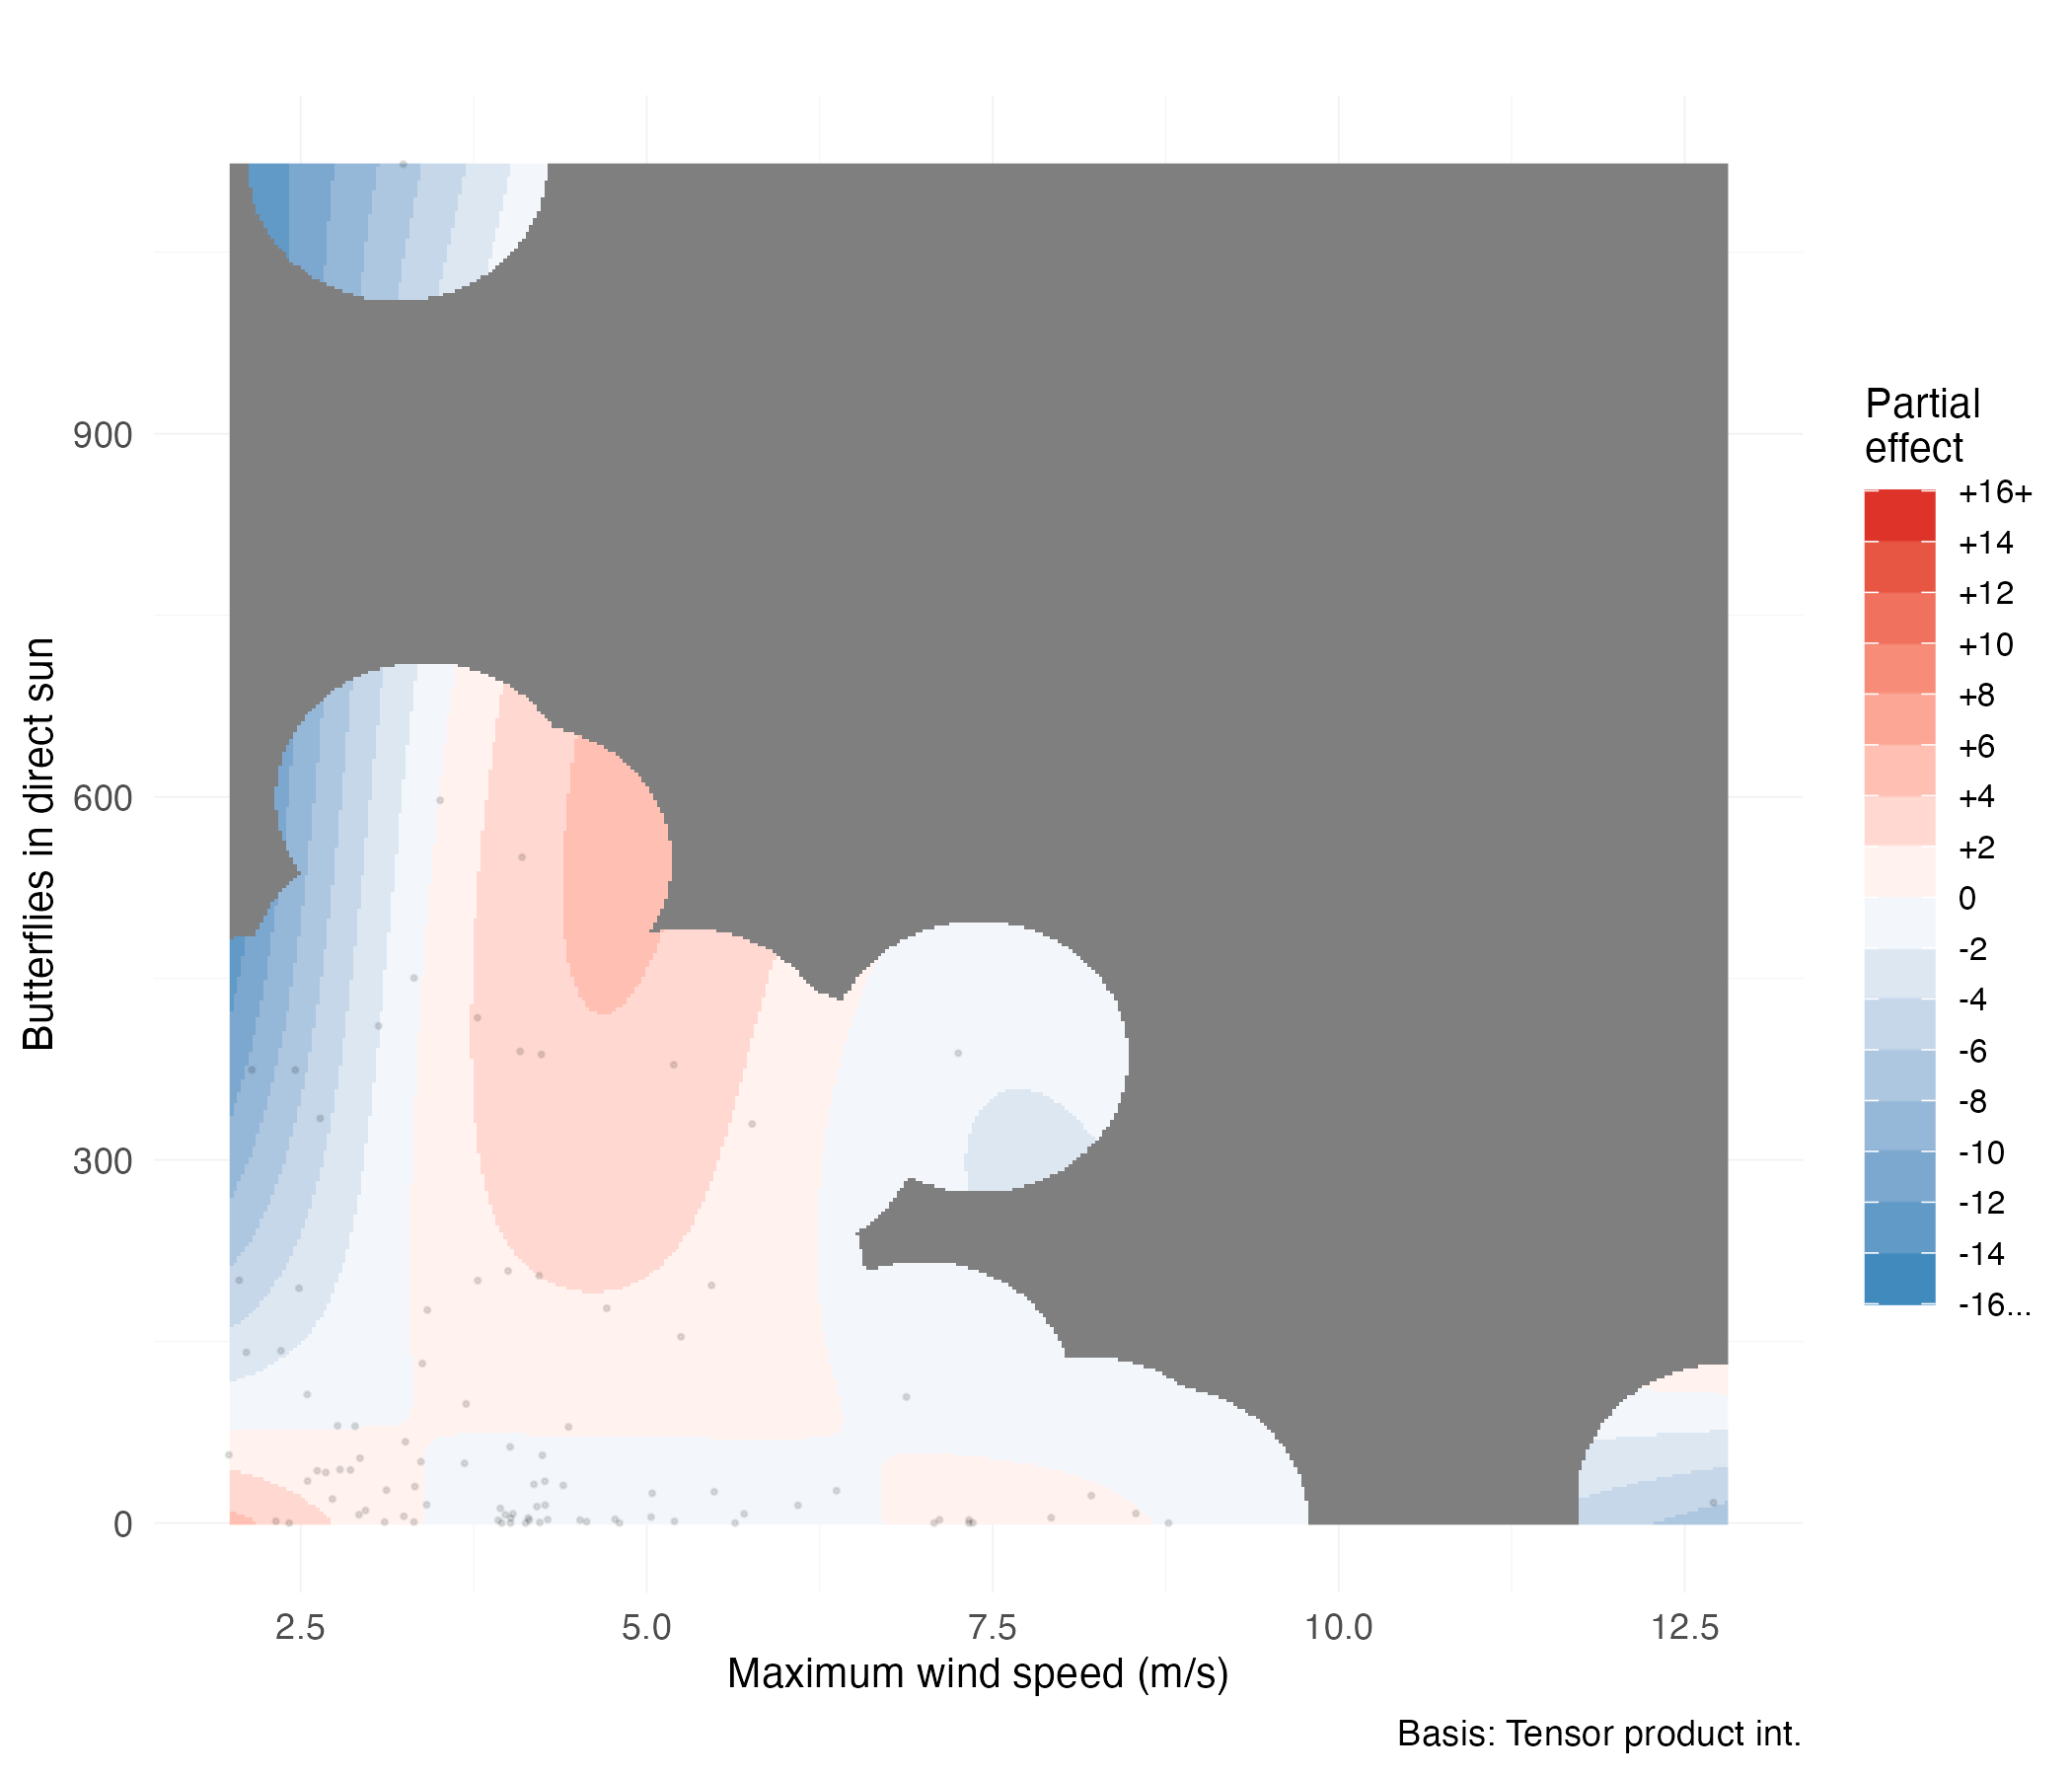
\includegraphics[width=0.8\textwidth]{supplemental/results/24hr/figures/interaction_wind_x_sun_binned.png}
    \caption{Tensor smooth interaction between maximum wind gust (m/s) and cumulative butterflies in direct sun on 24-hour cluster size changes. Color gradient indicates partial effect magnitude on square-root transformed scale (red = positive, blue = negative). Black points show observed data distribution. Gray regions indicate areas beyond reliable interpolation range. The interaction pattern mirrors that observed in the sunset-specific analysis, supporting the robustness of identified environmental relationships.}
    \label{fig:interaction_wind_sun_24hr}
\end{figure}